\documentclass[%
master,    % тип документа
natbib,      % использовать пакет natbib для "сжатия" цитирований
subf,        % использовать пакет subcaption для вложенной нумерации рисунков
href,        % использовать пакет hyperref для создания гиперссылок
colorlinks,  % цветные гиперссылки
%fixint,     % включить прямые знаки интегралов
]{disser}

\usepackage[
a4paper, mag=1000,
left=2.5cm, right=1cm, top=2cm, bottom=2cm, headsep=0.7cm, footskip=1cm
]{geometry}

\usepackage[intlimits]{amsmath}
\usepackage{amssymb,amsfonts}

\usepackage[T2A]{fontenc}
\usepackage[utf8]{inputenc}
\usepackage[english,russian]{babel}
\ifpdf\usepackage{epstopdf}\fi
\usepackage[autostyle]{csquotes}
\usepackage{rotating}
% Шрифт Times в тексте как основной
%\usepackage{tempora}
\usepackage{setspace}
\usepackage{mathtools}
% альтернативный пакет из дистрибутива TeX Live
%\usepackage{cyrtimes}
\usepackage{listings}
% Шрифт Times в формулах как основной
%\usepackage[varg,cmbraces,cmintegrals]{newtxmath}
% альтернативный пакет
%\usepackage[subscriptcorrection,nofontinfo]{mtpro2}

% Плавающие рисунки "в оборку".
\usepackage{wrapfig}
\usepackage{braket}
% Номера страниц снизу и по центру
%\pagestyle{footcenter}
%\chapterpagestyle{footcenter}

% Точка с запятой в качестве разделителя между номерами цитирований
%\setcitestyle{semicolon}

% Использовать полужирное начертание для векторов
\let\vec=\mathbf
%______________________________-
\usepackage{lipsum}

%\usepackage{titlesec}
%\usepackage{spacing}
%\titleformat{\section}[block]{\color{blue}\Large\bfseries\filcenter}{}{1em}{}
% Номера страниц снизу и по центру
\pagestyle{footcenter}
\chapterpagestyle{footcenter}

% Точка с запятой в качестве разделителя между номерами цитирований
%\setcitestyle{semicolon}



% Переопределение стандартных заголовков
%\def\contentsname{Содержание}
%\def\conclusionname{Выводы}
%\def\bibname{Литература}

\usepackage{geometry} % пакет для установки полей
\geometry{top=1.5cm} % отступ сверху
\geometry{bottom=2cm} % отступ снизу
\geometry{left=3cm} % отступ справа
\geometry{right=1.5cm} % отступ слева
\newcommand{\sectionbreak}{\clearpage}
\newcommand*{\No}{\textnumero}
\renewcommand{\Re}{\mathrm{Re}}
\renewcommand{\Im}{\mathrm{Im}}

\newcommand{\const}{\mathrm{const}}
\newcommand{\arccosh}{\mathrm{arccosh}}

\newcommand{\vF}{\mathbf{F}}
\newcommand{\ve}{\mathbf{e}}
\newcommand{\vk}{\mathbf{k}}
\newcommand{\vq}{\mathbf{q}}
\newcommand{\vp}{\mathbf{p}}
\newcommand{\va}{\mathbf{a}}
\newcommand{\vP}{\mathbf{P}}
\newcommand{\vK}{\mathbf{K}}
\newcommand{\vQ}{\mathbf{Q}}
\newcommand{\vA}{\mathbf{A}}
\newcommand{\vr}{\mathbf{r}}
\newcommand{\vR}{\mathbf{R}}

\newcommand{\vRR}{\boldsymbol{\mathcal{R}}}
\newcommand{\veps}{\boldsymbol{\varepsilon}}

\newcommand{\cA}{\mathcal{A}}
\newcommand{\cR}{\mathcal{R}}
\newcommand{\cM}{\mathcal{M}}
\newcommand{\cE}{\mathcal{E}}
\newcommand{\cJ}{\mathcal{J}}
\newcommand{\cT}{\mathcal{T}}
\newcommand{\cD}{\mathcal{D}}


%______________________________-
% Включать подсекции в оглавление
\setcounter{tocdepth}{2}

\graphicspath{{fig/}}

\begin{document}
\title{Моделирование нуклеосинтеза в звездах}
\maketitle
\tableofcontents
\section*{\centering Введение}
\addcontentsline{toc}{section}{Введение}
Данная работа рассматривает процесс синтеза ядер, а именно возникновение элементов в ходе эволюции нейтронной звезды. Преобразования, приводящие к появлению легких элементов (легче железа) известны и хорошо изучены. Распространенность элементов, расположенных в области за железом, относительно слабо зависит от массового числа A. Это свидетельствует об изменении механизма образования этих элементов.  Образование их в результате взаимодействия заряженных частиц сильно подавлено из-за кулоновского барьера. Фактор, который также необходимо принять во внимание, состоит в том, что большинство тяжелых элементов являются $\beta$-радиоактивными. По современным представлениям тяжелые элементы образуются в реакциях захвата нейтронов. Обычно различают быстрый (r) и медленный (s) процессы захвата нейтронов (от английских слов rapid и slow). Эти два механизма различаются отношением скорости захвата нейтронов (реакция (n, $\gamma$)) к скорости бета-распада. По современным представлениям примерно половина наблюдаемого количества элементов с A > 60 образуется в результате s-процесса. В настоящее время общепризнанно, что многие ядра тяжелее железа, включая все ядра тяжелее $^{209}Bi$, образуются в r-процессе путем быстрого последовательного захвата большого количества нейтронов. Главное условие - скорость захвата нейтронов должна быть больше скорости $\beta$-распада. 

Однако есть также некоторые элементы, возникновение которых не может происходить через эти процессы. Такие элементы являются обойденными. 

В данной работе, будут моделироваться реакции, приводящие к появлению обойденных ядер, а именно - столкновительный $\beta$-распад, с использование открытой библиотеки реакций REACLIB, в основе которой лежит построение сечения зависимостью от температуры по 7 параметрам. Данная библиотека уже включает в себя некоторый набор реакций, приводящий к появлению обойденных ядер, но в данной работе нас интересует исследование только влияние СБР на эволюцию системы. 

Основной целью работы является построение сечений для столкновительного $\beta$-распада для столкновении элементов с протоном, а также оценка влияния этих реакций на полученную распространенность элементов в результате всех процессов за промежуток времени.

Сам процесс моделирования будет выполняться с помощью открытой библиотеки SkyNet, написанную Jonas Lippuner с дополнение ее своим набором реакций.

\section{Нуклеосинтез Большого Взрыва}

\begin{figure}[h]
	\center{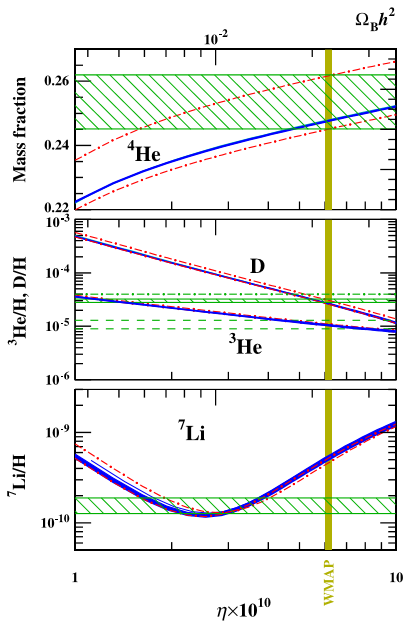
\includegraphics[width=0.7\linewidth]{2}}
	\caption{Вычисленная распространенность 4He, D, 3He и 7Li (синие линии) в зависимости от отношения барион-фотон $\eta$. Зеленые области - наблюдаемые концентрации, а желтая вертикальная полоса - наблюдаемое значение $\eta$. Вычисленные количества 4He, D и 3He согласуются с наблюдениями, но прогнозируется избыток 7Li в 4-5 $\sigma$. Это известная «литиевая проблема». Рисунок 1 из Cocetal. (2013)}
	\label{ris:Cocetal}
\end{figure}

Нуклеосинтез большого взрыва (BBN) произвел в основном водород ($\sim75\%$ общей массы) и гелий ($\sim25\%$) в период от первых десяти секунд до минуты после Большого взрыва, а также некоторое количество дейтерия, $^3H$e и $^7Li$ \cite{Tytler}. 13,8 тысяч световых лет позже химический состав Вселенной оставался около 75$\%$ H и 25$\%$ He, потому что создание более тяжелых элементов требует экстремальных физических условий. Интересно, что BBN является проблемой для моделирования, потому что он включает лишь небольшое количество ядер. В настоящее время существуют большие расхождения между результатами моделирование BBN и наблюдениями. Прогнозируемый дейтерий и распространенность 4He хорошо согласуется с наблюдениями, но модели BBN предсказывают большую распространенность 7Li на 4-5 $\sigma$ по сравнению с наблюдениями, см. рис. \ref{ris:Cocetal}. Это расхождение не до конца изучено и называется «литиевой проблемой». Предлагаемые причины включают систематические ошибки в наблюдениях численности 7Li, неизвестные или плохо измеренные ядерные свойства $^{7}Be$ и даже неизвестные физические процессы, не учтенные в стандартной модели.

\subsection{Горение в звездах малой массы}

\begin{figure}[h]
	\center{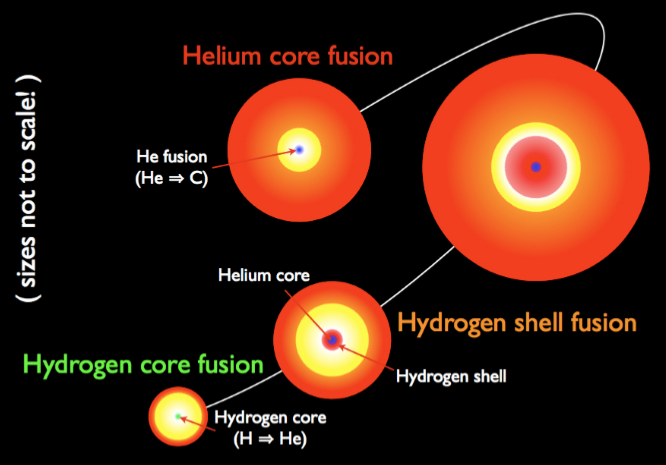
\includegraphics[width=0.7\linewidth]{3}}
	\caption{Изображение ранних этапов эволюции звезд. Звезда начинается со слияния	водорода с гелием. Когда водород в активной зоне истощен, ядро сжимается, что повышает температуру и запускает водородное слияние в оболочке вокруг гелиевого ядра. Это расширяет атмосферу звезды и превращает ее в красного гиганта. После сжигания водородного топлива ядро снова сжимается под действием силы тяжести, которая увеличивает температуру до той отметки, при которой синтез начинался. Рисунок из $https://www.nasa.gov/mission\_pages/$}
	\label{ris:evolution}
\end{figure}

Главное препятствие объединения гелия и водорода в тяжелые элементы - это сильное Кулоновское отталкивание между нуклидами, которые все положительно заряжены. Более того, стандартный способ слияния водорода это p-p цепь, включающая слабую реакцию $p + p \rightarrow d + e^+ + \nu_e$, которая имеет чрезвычайно малое сечение \cite{cauldrons}. Поэтому чрезвычайно высокие температуры ($\sim$ 10 MK) являются необходимым условием для преобразования водорода в гелий и гелий в более тяжелые элементы. Такие условия достигаются внутри звезд, где происходит ядерный синтез\cite{energy}, высвобождая энергию ядерной связи в виде тепла, удерживающую звезду от разрушения и заставляя ее излучать свет.

На рис. \ref{ris:evolution} изображены ранние стадии эволюции звезд. По определению, каждая звезда, по крайней мере, синтезирует водород в гелий внутри ядра. Звезды проводят большую часть своей жизни в этой фаза горения водорода. Как только запас водорода в ядре исчерпан, температура становится недостаточно высокой для сжигания гелия, поэтому ядро сжимается, потому что источник тепла от сжигания водорода уменьшается. Далее, поскольку ядро сжимается, оно нагревается, и температура становится достаточно высокой для горения водорода в оболочке вокруг гелиевого ядра. В этот момент атмосфера звезды быстро расширяется, и звезда входит в фазу красного гиганта. Когда водород в оболочке исчерпан и, если звезда достигла определенной массы ($\sim$ 0,5 $М_\odot$, например), ядро снова сжимается, то есть увеличивается температура и становится возможен тройной-альфа процесс, который  преобразует три частицы $^4He$ в $^{12}C$. Некоторые гелиевые сплавы также могут быть преобразованы с вновь созданным $^{12}C$, чтобы создать $^{16}O$, и, в принципе, он также может пойти дальше, производя $^{20}Ne$, $^{24}Mg$, $^{28}Si$ и т. д., которые называются альфа-элементами, потому что они являются определенным количество альфа-нуклидов, слитых воедино. Однако на практике реакция $^{16}O + \ ^4He \rightarrow \ ^{20}Ne$ протекает медленно, и поэтому сжигание гелия в основном производит $^{12}C$ и $^{16}O$ \cite{interiors}. Когда запасы гелия истощаются, температура ядра снова повышается за счет сжатия. Наибольшая температура, достигаемая в звезде, зависит от ее начальной массы. Если начальная масса выше $\sim 8 M_\odot$, то углерод и кислород могут быть сожжены, в противном случае звезда заканчивает свою жизнь как углерод-кислородный белый карлик. Если масса звезда представляет собой лишь несколько солнечных масс выше $8 M_\odot$, она может быть способна сжигать углерод, а затем стать белым карликом кислорода - то есть иметь неоновый цвет.

\subsection{Ядерное горение в тяжелых звездах}

\begin{figure}[h]
	\center{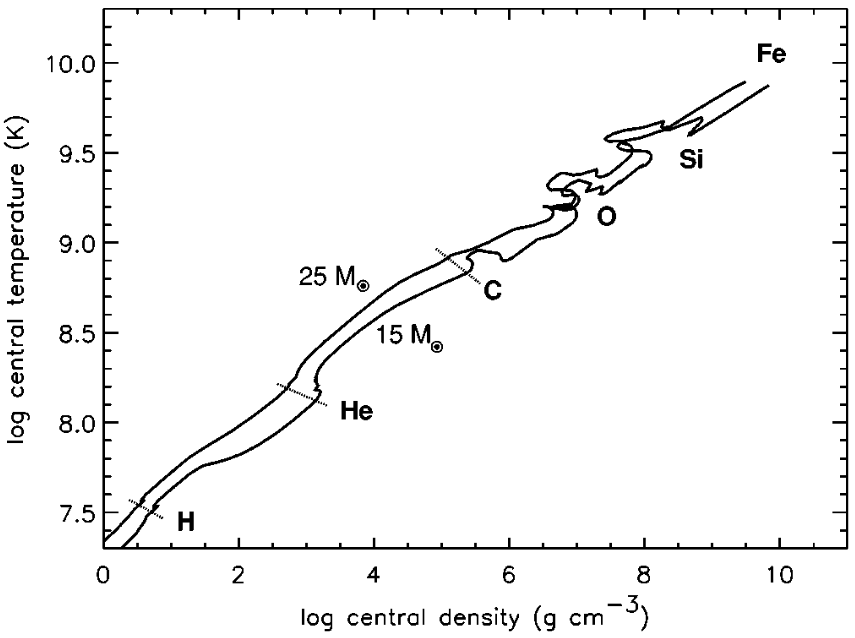
\includegraphics[width=0.7\linewidth]{4}}
	\caption{Центральная плотность и температура $15M_\odot$, а также $25M_\odot$ звездных моделей. По мере эволюции звезды центральная плотность и температура возрастают, последовательно воспламеняются водород, гелий, углерод, кислород и сгорает кремний \cite{massive}}
	\label{ris:massive}
\end{figure}

Звезды с начальной массой более $8 М_\odot$ проходят через несколько стадий горения. После каждого этапа, ядро сжимается под действием сил тяжести, поскольку ядерное топливо на этой стадии был исчерпано и, следовательно, источник ядерного тепла потерян. Поскольку ядро сжимаются, они нагревается, что позволяет начать следующую стадию горения, если температура достаточно высока. Это показано на рис \ref{ris:massive}, который показывает центральную плотность и температуру двухзвездной модели и областей, в которых происходят различные стадии горения. В фазе сжигания углерода существуют ряд различных реакции $^{12}C + \ ^{12}C$, но чаще всего наблюдается $^{20}Ne + \ ^{4}He$ и $^{23}Na + p$. Свободный протон может захватывать другие существующие ядра для создания не-альфа-элементов, а также $^{23}Na$, являющийся не-альфа-элементом, который могут быть преобразован в другие не-альфа-элементы. Гелий, полученный из сгорания углерода также сжигается как $^{12}C + ^{4}He \rightarrow \ ^{16}O$ или $^{16}O + \ ^{4}He \rightarrow \ ^{20}Ne$. Когда углерод истощается, ядро сжимается до тех пор, пока энергичные фотоны, формирующие хвост Распределения Планка не смогут фото-синтезировать $^{20}Ne$, что приводит к образованию свободных альфа-частиц, которые могут захватывать недиссоциированные $^{20}Ne$, чтобы сформировать около $^{24}Mg$. Реакция с низшим кулоновским барьером теперь $^{16}O + \ ^{16}O$, что в основном приводит к $^{28}Si + \ ^4Не$ и $^{31}P + p$ \cite{cauldrons}. Освобожденные альфа-частицы захватываются на $^{24}Mg$ и $^{28}Si$, чтобы сформировать $^{28}Si$ и $^{32}S$.

В конце сжигания кислорода, звездное ядро состоит в основном из $^{28}Si, \ ^{32}S$ и небольшого количества других ядер. Это является предпосылкой для окончательной фазы горения: сжигание кремния. Перед тем, как температура, требуемая для $^{28}Si + \ ^{28}Si$ достигается, кремниевые нуклиды разрушаются фото-диссоциацией, что снова создает источник для свободных альфа-частиц. Эти альфа-частицы захватываются последовательно, начиная с $^{28}Si$ для создания $\ ^{32}S, \ ^{36}Ar, \ ^{40}Ca, \ ^{44}Ti, \ ^{48}Cr, \ ^{52}Fe$ и $^{56}Ni$, что называется альфа процессом или альфа-лестницой, которая происходит в течении дня. Поскольку температура во время сжигания кремния настолько высока ($\sim$ 3,5 ГК), нуклиды, более тяжелые, чем кремний, также могут быть фото-диссоциированны. Результатом являются такие реакции, как  $^{28}Si + \ ^4He \rightarrow \ ^{32}S$, которые находятся в равновесии с их обратными реакции. Таким образом, существует группа нуклидов, а именно нуклидов с $28 \le A \le 62$, свободные альфа-частицы, нейтроны и протоны, находящихся в равновесии друг с другом. Это состояние называется квазиравновесным (QSE) и отличается от NSE тем, что не все нуклиды находятся в равновесии друг с другом. В частности, $^{12}C, \ ^{16}O, \ ^{20}Ne$, и $^{24}Mg$ не являются частью группы QSE \cite{qse}.

Однако сжигание кремния могут производить только нуклиды вплоть до атомного массового числа от А = 56, так как энергия связи на нуклон (протоны и нейтроны) достигает максимума при этом массовом числе. Поэтому более тяжелые нуклиды связаны слабее, что означает, что нужно добавить энергию, для обеспечения слияние за пределами A = 56. Другими словами, как только все значимые элементы (до $^{56}Ni$) в ядре массивной звезды сожжены, сердцевина звезды будет состоять из ядерной пыли, которая не может гореть и звезда теряет свой основной источник тепла. Ядро удерживается от коллапса давлением вырождения электронов, но как только масса ядра превышает эффективную массу Чандрасекара, происходит коллапс ядра, вызывающий CCSN (например, Woosley et al., 2002). Масса Чандрасекара ($\sim 1,4 М_\odot$) является теоретической максимальной масса белого карлика, поддерживаемого только лишь давлением вырождаемости электронов. Однако до того, как железное ядро достигнет массы Чандрасекара, происходит захват электронов нуклидами, которые удаляют электроны и, следовательно, поддерживающее давление, что приводит к коллапсу ядра до того, как оно достигнет массы Чандрасекара. Максимальная масса железного ядра до начала коллапса называется эффективной массой Чандрасекара \cite{massive}. Поскольку звездный синтез по большей части производит альфа-элементы, неудивительно, что мы наблюдаем альфа-элементы, более распространенными, чем другие нуклиды с массовым числом ниже железа (см. рис. \ref{ris:abundancies}).

\begin{figure}[h]
	\center{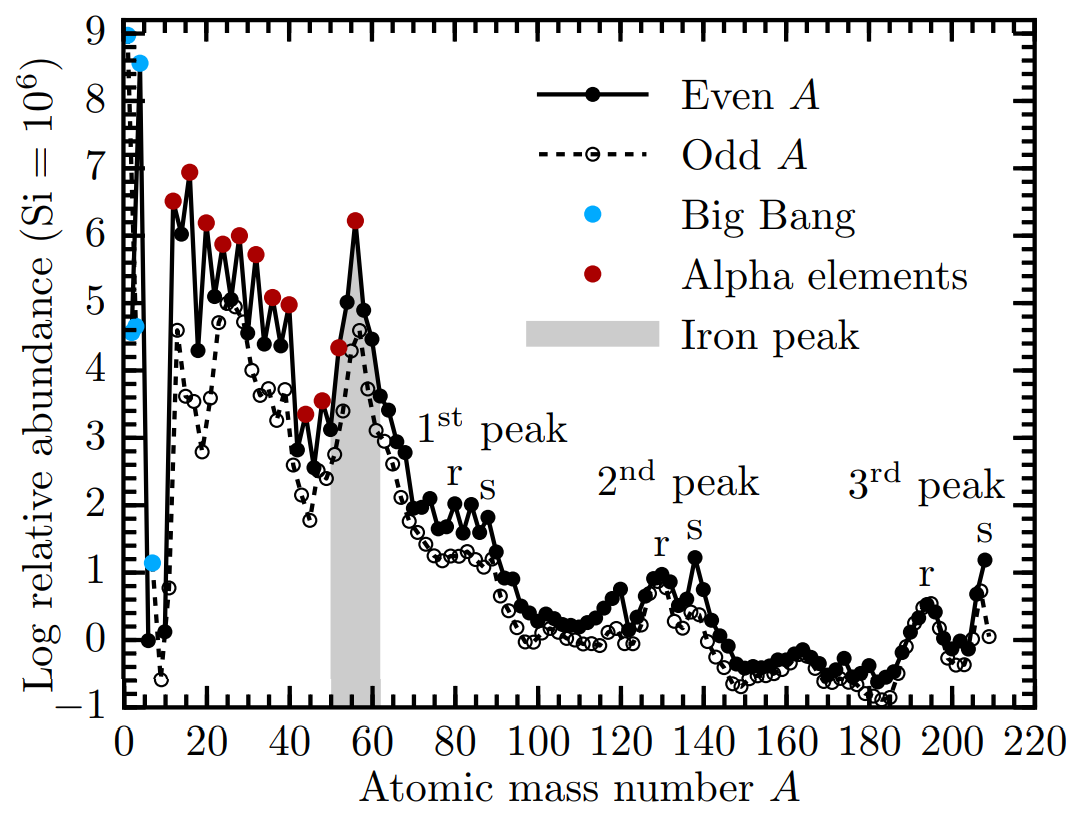
\includegraphics[width=0.7\linewidth]{1}}
	\caption{Наблюдаемая распространенность в нашей солнечной системе в зависимости от массового числа А. Самые легкие элементы были созданы в «Большом взрыве». Слияние в звездах преимущественно создает альфа-элементы \cite{abundancies}}
	\label{ris:abundancies}
\end{figure}

\subsection{Пик железа}

Выше температуры (~5GK), реакции слияния уравновешиваются обратной реакцией фотодиссоциации, что означает, что реакция плавления $N$ нейтронов и $Z$ протонов в нуклиде $(N, Z)$ уравновешивается реакцией расщепления в нуклиде $(N, Z)$ на $N$ свободных нейтронах и $Z$ свободных протонах. Такое состояние называется ядерное статистиче (NSE). Когда материя находится в состоянии NSE, весь состав, т. е. концентрация каждого вида ядра, полностью определяется температурой, плотности и электронной частью $Y_e = n_p/(n_p + n_n)$, где $n_p$ - общая плотность протонов (свободных или внутри нуклидов), а $n_n$ - аналогичное значение для нейтронов \cite{nse}.

Такие условия достигаются в сверхновой типа $Ia$, где белый карлик, состоящий в основном из углерода и кислорода, подвергается термоядерному взрыву. Последующее нагревание заставляет материю перейти в состояние NSE, которое порождает пики железа нуклидов, которые останутся присутствовать в системе после снижения температуры.

\begin{figure}[h]
	\center{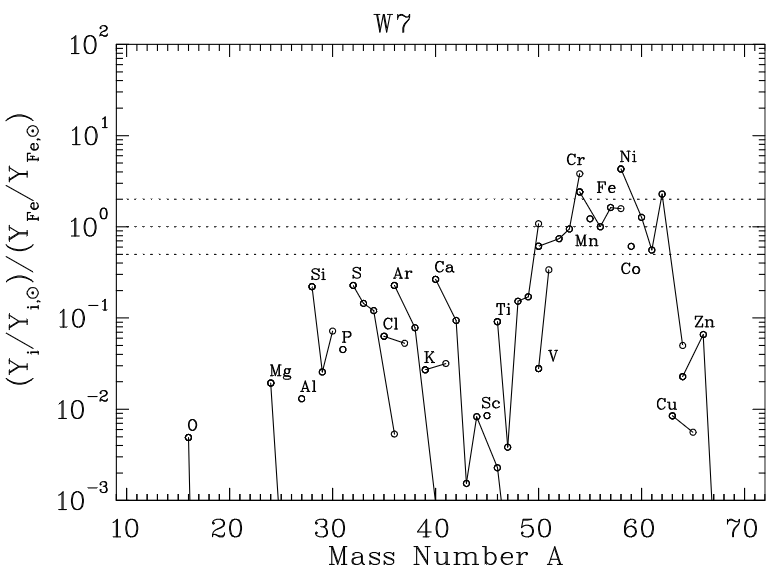
\includegraphics[width=0.7\linewidth]{5}}
	\caption{Конечные показатели концентрации в модели сверхновой типа $Ia$. В основном наблюдаются элементы вблизи железного пика, а также некоторые тяжелые альфа-элементы (кремний, сера, аргон, кальций и титан)}
	\label{ris:iron-abu}
\end{figure}

Рисунок \ref{ris:iron-abu} показывает конечную концентрацию из модели сверхновой звезды типа $Ia$ \cite{iron-abu}. Тип $Ia$ сверхновых вносит значительный вклад в формирование пика железа вместе с горением кремния во время CCSNe и медленного захвата электронов в тяжелых звездах.

\subsection{Нуклеосинтез за пиком железа}
Поскольку процесс слияния становится эндотермическим для A $\ge$ 56, а кулоновский барьер становится непреодолимо большим, требуется другой процесс для создания элементов за пиком железа. Этот процесс представляет собой захват нейтронов, который остается экзотермическим до тех пор, пока энергия связи нейтронов $Q_n$ является большой для богатых нейтронами ядер. В некоторой точке, $Q_n$ настолько мала ($~\sim1 \text{МэВ}$), что показатель фоторасщепления (фотонный выброс нейтрона из ядра) так же велик, как и показатель захвата нейтронов, и поэтому нет дополнительных нейтронов, связанными с ядром. Момент, в который это происходит называется нейтронной капельной линией (!!! neutron drip line) и, как правило, составляет 10-20 нейтронов, превышающих наиболее богатый нейтронами стабильный изотоп \cite{cauldrons}. Точное положение нейтронной капельной линии зависит от температуры и плотности нейтронов. Очевидно, что Кулоновский барьер  для захвата нейтронов отсутствует, поскольку нейтроны имеют нейтральный заряд.

Как только ядро захватывает нейтрон, оно может оставаться стабильным, и в этом случае оно может захватить другой нейтрон, но в большинстве случаев новый нуклид будет неустойчивым к $\beta$-распаду.

Важным отличием является то, что время $\tau\beta$ для $\beta$-распада короче или длиннее чем время $\tau_n$ для захвата нейтронов. Если $\tau_\beta << \tau_n$, то каждое неустойчивое ядро, созданное захватом нейтронов, распадется до стабильного ядра, прежде чем у него появится шанс захвата другого нейтрона. Следовательно, процесс захвата нейтронов медленный по сравнению с $\beta$-распадом, и поэтому это называется s-процессом (slow). S-процесс никогда не дестабилизирует более одного ядра и, следовательно, протекает вдоль области устойчивости (область на карте нуклидов, где ядра стабильны, обозначена квадратами на рис. \ref{ris:6}). Если, с другой стороны, $\tau_\beta \gg \tau_n$, то есть достаточно времени для множественных захватов нейтронов до первого $\beta$-распада. Это называется r-процессом, поскольку захват нейтронов происходит быстро. В этом случае нуклеосинтез протекает вдоль нейтронной капельной линии, но он вынужден дождаться $\beta$-распада в этой точке.

\begin{figure}[h]
	\center{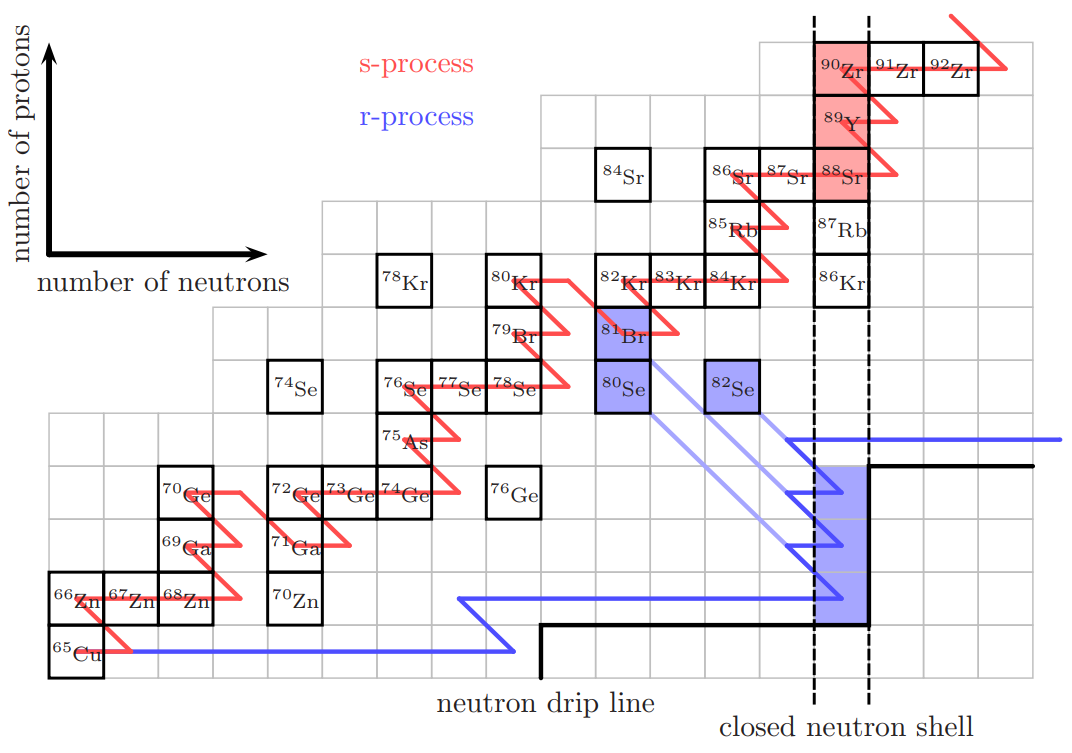
\includegraphics[width=0.7\linewidth]{6}}
	\caption{Схематическое представление s- и r-процесса на участке диаграммы нуклидов. S-процесс (красный) проходит вдоль долины устойчивости и r-процесс (синий) вдоль линии капельного потока нейтронов. На закрытой нейтронной оболочке N = 50 сечение захвата нейтронов падает на несколько порядков, что приводит к накоплению материала, который производит двух-пиковые характеристики, показанные на рисунке 1.1}
	\label{ris:6}
\end{figure}

На рис. \ref{ris:6} схематично показаны пути s- и r-процессов на участке диаграммы нуклидов. Если ядро имеет определенной количество нейтронов, называемое магическим числом, то нейтроны могут быть расположены в замкнутой оболочке, которая энергетически очень благоприятна и резко уменьшает сечение захвата нейтронов. Это показано на рисунке 1.6 при N = 50. Когда r-процесс достигает замкнутой нейтронной оболочки, ему приходится ждать, пока произойдет несколько $\beta$-распадов могут протекать мимо закрытой нейтронной оболочки. Поэтому материал будет накапливаться там, где нейтронная капельная линия пересекает замкнутую нейтронную оболочку, обозначенную квадратами на рис. \ref{ris:6}. Поскольку эти нуклиды все нестабильны, они в конечном итоге распадаются до состояния устойчивости когда все свободные нейтроны будут захвачены, а избыток материала, который был получен на закрытой нейтронной оболочке, приведет к пику обилия в массе, где нуклиды имеют меньше нейтронов, чем магическое число (потому что некоторые нейтроны распались на протоны). Аналогичным образом, когда s-процесс пересекается с закрытой нейтронной оболочкой, также будет избыток материала но не потому, что s-процесс должен ждать дополнительных $\beta$-распадов (напомним, что $\beta$-распады всегда происходят намного быстрее, чем захват нейтронов s-процесса). Материя накапливается на закрытой нейтронной оболочке, поскольку сечение захвата нейтронов на один-два порядка меньше, чем для соседних нуклидов. Таким образом, s-процесс будет порождать пики обилия в тех массах, где число нейтронов - это в точности магическое число, которое является большей массой, чем пики, образуемые r-процессом. Наиболее важные магические числа это N = 50; 82; 126, которые приводят к пикам распространенности при приблизительно A = 80; 130; 194 для r-процесс и около A = 88; 138; 208 для s-процесса. Когда мы исследуем r-процесс, мы всегда сравниваем предполагаемое обилие с паттерном солнечного r-процесса. Оказывается, что вклад r-процесса является универсальным и относительное обилие в Солнце аналогично относительному обилию, наблюдаемому в гало звезд с недостатком металла. Обилия r-процесса из пяти таких звезд показаны на рис. \ref{ris:8}. Звезды с ореолам, бедными металлами, сформировались на ранней стадии жизни нашей галактики, и поэтому мы ожидаем, что они не будут значительно обогащены тяжелыми элементов, созданных s-процессом, поскольку у него не было достаточного времени для образования этих звезд. Поэтому любая реалистическая модель нуклеосинтеза r-процесса должна воспроизводить обилия солнечного r-процесса.

\begin{figure}[h]
	\center{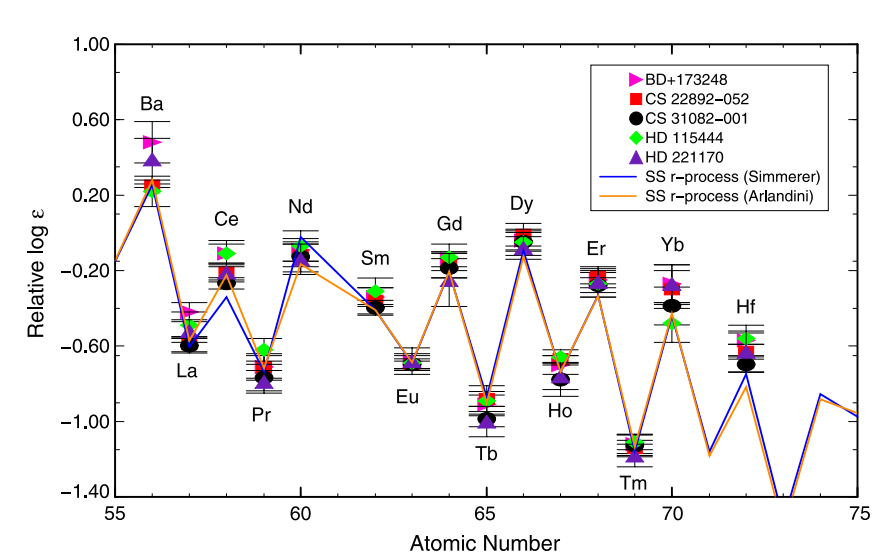
\includegraphics[width=0.7\linewidth]{8}}
	\caption{Наблюдаемые обилие некоторых тяжелых элементов в пяти металлически-бедных ореолах  звезд. Распространенности нормируются через европиум. Все звезды имеют практически одинаковые относительные распространенности, и эта картина также согласуется с тем, что наблюдается в солнечной системе (линии). Ожидается, что эти звезды не будут обогащены s-процессом нуклеосинтеза, потому что они образовались вскоре после образования галактики  \cite{new-abu}}.
	\label{ris:8}
\end{figure}

Наконец, некоторые авторы также рассматривают процесс промежуточного захвата нейтронов, называемый i-процесс, между медленным и быстрым процессами. I-процесс протекает на богатой нейтронами стороне, и дестабилизирует до пяти нуклидов. S-процесс и/или i-процесс происходят внутри звезды с низкой массой асимптотической гигантской ветви (AGB) ($1.5 \le M/M_\odot \le 3$), а также более массивных звездах, которые, как правило, имеют сильные звездные ветра, которые выбрасывают некоторые из вновь созданных тяжелых элементов в межзвездную среду. Реакции $^{13}C + \ ^4He \to \ ^{16}O + n$ и $^{22}Ne + \ ^4He \to \ ^{25}Mg + n$ приводят к появлению свободных нейтронов. Астрофизические условия r-процесса остаются открытыми вопросами и являются предметом следующего раздела.

\subsection{Возможные места r-процесса}

Для r-процесса требуется очень богатая нейтронами среда. Было предложено множество мест, в которых могут быть достигнуты правильные условия для r-процесса. К ним относятся ударные или струйные выбросы в сверхновых, богатых нейтронами, неоднородные космологии Большого Взрыва, выбросы от коалесценции и приливного разрушения бинарных нейтронных звезд, выбросы взрывчатого гелия или сжигание углерода, вспышки гелиевых ядер в звездах с низкой массой, или аккреционные диски нейтронной звезды. Основываясь на наблюдениях европия в звездах с небольшим содержанием металла и галактических моделях химической эволюции, Мэтьюз и Коуэн (1990) пришли к выводу, что CCSN были наиболее вероятным местом протекания r-процесса \cite{places}. Недавние исследования показывают, что CCSN и слияние нейтронных звезд являются единственными жизнеспособными кандидатами на места протекания r-процесса \cite{sites}.

\subsection{Распространенность в солнечной системе}
Крайне сложно получить образцы материи из мест, отличных от земной коры. \textit{Apollo} и \textit{Luna} принесли образцы с луны, а позже такие космические аппараты, как \textit{Stardust}, \textit{Genesis}, и \textit{Hayabusa} успешно доставили образцы из близлежащих астероидов и космической пыли на Землю. Однако подавляющее большинство внеземных материалов, доступных для химических анализов получены от метеоритов, которые падают на поверхность Земли. Поэтому, чтобы определить состав звезд и других астрофизических	 объектов, мы ограничимся изучением линиями поглощения и излучения, формирующими эти объекты, а также распространенность элементарных частиц \cite{shaviv}. Линии поглощения (!!!Absorption) в солнечном спектре были впервые обнаружены в начале XIX век. Тем не менее, применение им нашли только 100 лет спустя, после развития квантовой механики, которая утверждает, что линии поглощения могут использоваться для количественного определения распространенности элементов на солнце.

На рис. \ref{ris:abundancies} показаны наблюдаемые распространенности в нашей солнечной системе в зависимости от массового числа А. Нуклиды с четным массовым числом как правило более многочисленными, чем нуклиды с нечетным массовым числом. Из-за спинового спаривания нуклонов нуклид с четным число нейтронов и протонов (следовательно, четное A) является более связанным, чем нуклид с нечетным числом нейтронов или протонов (следовательно, нечетное А) \cite{zur}. Нуклиды с нечетным числом и нейтронов, и протонов (отсюда и четное A), имеют еще более слабую связь поскольку ни все нейтроны, ни все протоны не могут быть спин-парными. Поэтому неудивительно, что существует только несколько нечетных-нечетных нуклидов, которые являются стабильными или долгоживущими: $^2H$, $^6Li$, $^{10}B$ и $^{14}N$ стабильны, а $^{40}K$, $^{50}V$, $^{138}La$ и $^{176}Lu$ являются единственными нечетные-нечетные нуклиды с периодом полураспада не менее 1 миллиона лет. Существует ряд различных процессов нуклеосинтеза, которые доминируют в различных диапазонах масс. Очень легкие нуклиды (A <8) были получены сразу после Большого взрыва, некоторое количество $^4He$, а также большинство нуклидов в диапазоне $12 \le A \le 56$ являются результатом гидростатического ядерного горения в звездах, значительная часть пика железа ($50 \lesssim A \lesssim 62$) производится элементами, входящими в ядерное статистическое равновесие, а затем охлаждающимся.

\subsection{Коллапс ядра сверхновых}
После коллапса железного ядра массивной звезды образуется прото-нейтронная звезда (ПНС). Эта ПНС делептонизирует, чтобы в конечном итоге сформировать нейтронную звезду. Этот процесс испускает порядка $10^{53}$ эрг энергии связи в виде нейтрино. Большое облучение нейтрино приводит к горячему ветру с поверхности ПНС, называемому ветром, управляемым нейтрино \cite{neutrino}. Ранние симуляции этого ветра показывали, что в некоторых случаях они могут иметь хорошие условия для r-процесса.

Однако последние исследования нуклеосинтеза r-процесса в ветрах с участием нейтрино показали, что маловероятно, что r-процесс полностью (получение нуклидов до третьего пика, см. рис. \ref{ris:abundancies} протекает в этих условиях, поскольку ветер, похоже, недостаточно богат нейтронами. Получается, что только слабая версия r-процесса (получение тяжелых элементов до $A \sim 130$) может происходить в ветре с нейтрино от CCSNe.

Однако существует еще один процесс, так называемый «$\nu р$-процесс», который может создавать нуклиды до $А \sim 110$ в насыщенном протоннами ветре с участием нейтрино. В горячем, богатом протонами ветре, захват протонов создает богатые протоном ядра, но прекращается при $^{64}Ge$, который имеет долгий $\beta$ - период полураспада ($\sim 64$с) в масштабе времени ($\sim 10$с) и малое сечение захвата протонов. $\nu p$-процесс может пройти через этот $^{64}Ge$ барьер путем преобразования свободного протона в нейтрон посредством электронного антинейтринного захвата. Реакция $^{64}Ge + n \to \ ^{64}Ga + p$ намного быстрее, чем захват протонов на ${64}Ge$ и позволяет нуклеосинтезу преодолеть A = 64 с последующими захватами протонов

Наконец, определенный редкий тип CCSNe может иметь возможность обеспечивать полный r-процесс. Если звезда-предшественник имеет сильное магнитное поле, и ее ядро вращается быстро, тогда взрыв сверхновой может приводиться в действие магнитороциональными процессами (возможно магнитореформационная неустойчивость), которые могли создать биполярную струю. Возможно, что в этой струе имеет место r-процесс нуклеосинтеза, который создает все тяжелые элементы до третьего пика. Однако, из-за огромного магнитного поля и быстрого вращения, требуемого в этом типе суперновых, ожидается, что только малая доля ($\lesssim 0.1 \%$) из всех CCSNe приводит к созданию магниторотационной сверхновой.

\subsection{Слияние нейтронных звезд}

Поскольку обычный CCSN, скорее всего, не может произвести полный r-процесс, остается только слияние нейтронных звезд как единственное жизнеспособное место для нуклеосинтеза r-процесса. Мы знаем, что в нашей галактике существуют бинарные системы нейтронных звезд, и, что их орбита сокращается из-за излучения гравитационной волны, что приведет в результате к объединению двух нейтронных звезд. Множество групп провели гидродинамическое моделирование слияния двух нейтронных звезд или слияние нейтронной звезды и черной дыры. Такие слияния могут выбрасывать богатый нейтронами материал через различные процессы. Существует два типа динамических выбросов, которые запускаются незадолго до или во время слияния. Поскольку две нейтронные звезды приближаются друг к другу или одна нейтронная звезда приближается к своей черной дыре, нейтроная звезда(ы) деформируется и разрушается, что создает поток материи нейтронной звезды, выброшенный в космос и несвязанный с системой. Этот тип выброса относится к приливным хвостам. Пример показан на рисунке \ref{ris:11}. Второй тип динамических выбросов - сжатие материи при столкновении между двумя нейтронными звездами. Этот тип динамических выбросов происходят только при слияниях нейтронная звезда - нейтронная звезда (NSNS) \cite{nsns}. Масса динамического выброса находится от $10^{-4}$ до нескольких $\times 10^{-2}$ масс Солнца и распределение электронной доли колеблется от $Y_e \sim$ 0.05-0.45 в случае бинарных нейтронных звезд. Черные дыры-нейтронные звезды могут выбросить порядка $\sim 0.1 М_\odot$, но только если черная дыра имеет такую же массу, как нейтроная звезда и имеет довольно высокий уровень вращения. Иначе, как правило, нет выброса вообще, потому что нейтронная звезда разрушается внутри горизонта событий черной дыры. Доля электронного выброса от слияния BHNS обычно ниже 0,2.

\begin{figure}[h]
	\center{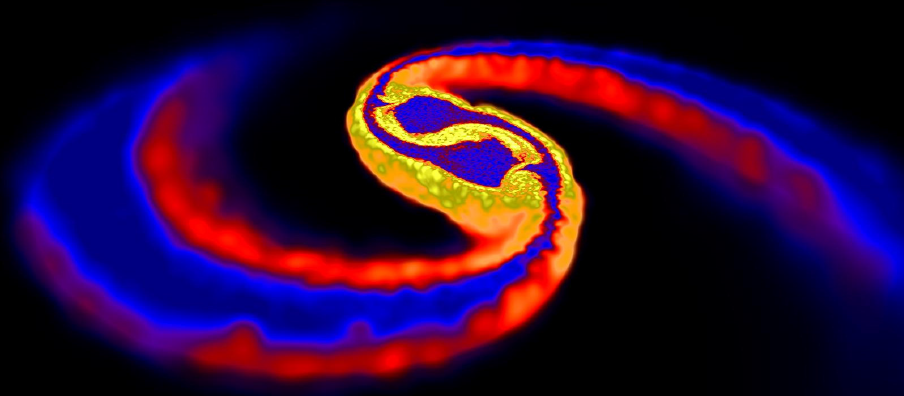
\includegraphics[width=0.7\linewidth]{11}}
	\caption{Плотностный рендеринг моделирования слияния двойных нейтронных звезд. Темные центральные капли - это две нейтронные звезды перед слиянием. Динамические выбросы богатого нейтронами вещества в виде двух приливных хвостов отчетливо видны. Этот материал является несвязанным, а также в нем происходит r-process. Рисунок из http://users.monash.edu.au/~dprice/research/nsmag}
	\label{ris:11}
\end{figure}

Слияние нейтронных звезд может привести к дополнительным оттокам после слияния. В большинстве случаев вокруг центрального компактного объекта, который является либо черной дырой, либо горячей гипермассивной нейтронной звездой (HMNS) образуется аккреционный диск или тор. Время жизни HMNS до того, как оно схлопнется до черной дыры, колеблется от нескольких миллисекунд до более 30 мс. Если есть HMNS, она будет излучать нейтрино. Горячий аккреционный диск также охлаждается через излучение нейтрино. Это может привести к ветру с нейтрино с поверхности диска. Отток с диска также может быть вызван вязким нагревом и альфа-рекомбинацией на диске. Поскольку этот отток происходит в более поздние времена, излучение нейтрино имеет достаточно времени для значительного повышения электронной доли в оттоке, так что большинство симуляций обнаруживают $Y_e \sim 0. 2 - 0.45$ с несколькими $\times 10^{-3} M_\odot$ выбрасываемыми в эти оттоки.

Поскольку выбросы от слияния нейтронной звезды настолько богаты нейтронами,  r-процесс может легко создать все элементы до $A \sim 250$, что выходит за пределы третьего пика. По факту, во время r-процесса нуклеосинтеза образуются еще более тяжелые нуклиды (A > 300) однако эти нуклиды нестабильны для деления (как спонтанные, так и нейтронно-индуцированные). Их продукты деления быстро захватывают больше нейтронов, растут до A > 300, а затем делятся сами собой. Этот так называемый цикл деления продолжается до тех пор, пока нейтроны не будут исчерпаны. Замечательный результат заключается в том, что окончательная картина обилия r-процесса очень устойчива к вариациям в детальных свойствах выброса. Если цикл деления начался, то конечная численность не будет зависеть от точного числа циклов. Рисунок 1.13 (рис. 4 от Korobkin et al., 2012) показывает результат r-процесса нуклеосинтеза в различных слияниях NSNS и BHNS. Все сценарии слияния производят по существу идентичные конечные распространенности, демонстрируя тем самым устойчивость r-процесса в слияниях нейтронных звезд.


\subsection{Химическая эволюция галактики}


\section{Столкновительный $\beta$-распад}
Данный процесс является одним из процессов, приводящих к появлению обойденных ядер.

Обойдённые ядра - устойчивые атомные ядра, лежащие в стороне от всех возможных путей образования тяжёлых ядер из более лёгких в процессе последовательного захвата последними нейтронов \cite{reactions}. Распространённость обойденных ядер, как правило, примерно на два порядка величины ниже, чем у близких к ним ядер, лежащих на пути нейтронного захвата. К таковым относятся: $^{74}Se$, $^{78}Kr$, $^{80}Kr$, $^{84}Sr$, $^{92}Mo$, $^{94}Мо$, $^{96}Ru$, $^{98}Ru$, $^{102}Pd$, $^{106}Cd$, $^{108}Cd$, $^{113}In$, $^{112}Sn$, $^{114}Sn$, $^{115}Sn$, $^{120}Te$, $^{124}Xe$, $^{126}Xe$, $^{130}Ba$, $^{132}Ba$, $^{136}Ce$, $^{138}Ce$, $^{144}Sm$, $^{152}Gd$, $^{152}Dy$, $^{158}Dy$, $^{162}Er$, $^{164}Er$, $^{168}Yb$, $^{174}Hf$, $^{180}W$, $^{184}Os$, $^{190}Pt$, $^{196}Hg$ \cite{role}.

Столкновительный $\beta-$распад стабильных ядер, инициируемый их кулоновскими столкновениями с другими ядерными частицами звездной среды, может быть основой модели процесса синтеза обойденных ядер.
Проблема их синтеза на основе физического механизма захвата нейтронов ($s-$ или $r-$процесса) состоит в прерывании цепочки последовательных $\beta-$распадов на $\beta$-стабильном ядре $(A,Z)$.

Процесс СБР стабильных ядер, о котором говорилось выше, для нуклидов главной последовательности предоставляет еще одну возможность преодолеть энергетический порог и осуществить переход 
$$(A,Z) \xrightarrow[]{\beta^-} (A,Z + 1),$$
открывая путь к последующему естественному $\beta$-переходу
$$(A,Z+1) \xrightarrow[]{\beta^-} (A,Z + 2)$$

Может оказаться, что при этом малость сечений для процесса такого рода уже не будет играть особой роли, если будут не малы плотность вещества в недрах звезды и временная протяженность квазиравновесной стадии звездной эволюции.

Расчеты показывают, что модель синтеза обойденных элементов в звездном веществе на этапе квазиравновесной стадии, основанная на явлении СБР стабильных ядер главной последовательности, качественно, а в ряде случаев и количественно, способна воспроизвести нерегулярный ход кривой относительной распространенности обойденных ядер. Этот факт можно расценивать как косвенное свидетельство в пользу реальности явления столкновительного $\beta$-распада стабильных ядер \cite{tak}.

В случае столкновительного $\beta$-распада возможно несколько видов процессов, а именно: протон-ядерные, ядро-ядерные и процесс, стимулированный нейтронами. Рассчитанные сечения для протон-ядерных и ядро-ядерных оказались невелики (менее $10^{-50}cm^2$), и процесс пока не доступен для прямого наблюдения, но при помощи программного обеспечения, позволяющего моделировать данные процессы мы можем оценить влияние их на конечные распространенности элементов \cite{tak_article}. Наряду с кулоновскими столкновениями ядер можно предложить механизм СБР, не связанный с кулоновскими силами и в то же время незамаскированный возможным появлением продуктов $\beta$-распада за счет ядерных реакций. Речь идет о процессе СБР ядра, стимулированном столкновениями с нейтронами.

Данная работа рассматривает в первую очередь влияние протон-ядерного столкновения на процессы, протекающие в нейтронных звездах, а именно r-process, так как концентрация протонов при этом достаточно велика, чтобы это влияние оказалось существенным. 

\subsection{Дифференциальное сечение  процесса столкновительного
	$\beta$-распада ядер в кулоновском поле отталкивания.}

Рассмотрим нерелятивистское столкновение двух ядер $(A,Z)$ и $(A',Z')$,
первое из которых для процесса $\beta^-$-распада - материнское ядро, а второе
- столкновительный партнер (для простоты он будет считаться
бесструктурным).
Дифференциальное сечение процесса столкновительного $\beta$-распада
нуклида $(A,Z)$ можно  представить в виде:
\begin{eqnarray}\label{ds}
&&d\sigma^{(col)}_\beta={2\pi\mu\over{\hbar^2k_i}}\sum_{\beta_f}{\left| \bra{f} H^{(\beta^-)}
	\ket{i}\right|}^2{d^3 K_f\over{(2\pi)^3}}{d^3 k_f\over{(2\pi)^3}}
{d^3 p_e\over{(2\pi\hbar)^3}}{d^3 p_\nu\over{(2\pi\hbar)^3}}\times\nonumber\\
&&\times\;\delta\left({\hbar^2 K_i^2\over{2 M}}+{\hbar^2 k_i^2\over{2\mu}}-{\hbar^2 K_f^2\over{2 M}}-
{\hbar^2 k_f^2\over{2\mu}}-E_e-E_\nu-\Delta-\Delta_f\right).
\end{eqnarray}
Здесь $\ket{i}$ и $\ket{f}$ - волновые функции начального и конечного состояний
столкновительной системы,
$\hbar \vec K_s$ и $\hbar \vec k_s$ - ее полный и относительный импульсы
в $s$-том состоянии ($s=i$ или $f$),
$\vec p_e$ и $\vec p_\nu$ - импульсы бета-электрона и антинейтрино,
$E_e$ и $E_\nu$ - их энергии,
$\Delta$ - пороговая энергия, определяемая разностью энергий связи
дочернего и материнского ядер (для $\beta$-стабильного ядра $\Delta>0$),
$\Delta_f$  - энергия состояния дочернего ядра, отсчитанная от
основного (см. рис.\ref{SH}),
$М$ и $\mu$ - полная и приведенная массы системы.
$\delta$-функция выражает закон сохранения энергии в процессе СБР.
Оператор ядерного бета-перехода  $H^{(\beta^-)}$ имеет вид \cite{aiz}:
\begin{eqnarray}\label{nH^beta}
H^{(\beta^-)}\approx {{1}\over{\sqrt{2}}}\sum_{j=1}^{A} \exp{( -i \vec q_\beta \vec r_j)}
(\tau_+)_j ( i g_v b_4 - g_a\, \vec b\, \vec \sigma_j ),
\end{eqnarray}
где $\vec r_j$ -- координата $j$-го нуклона;
$g_v$ и $g_a$ - векторная и псевдовекторная константы слабого
взаимодействия;
$\tau_+~=~(~\tau_1~+~i~\tau_2)/2$, $\;\tau_k,\sigma_k$ - операторы Паули;
$b_\lambda=i ( \bar u_e \gamma_\lambda \omega_\nu), u_e, \omega_\nu$ - лептонные
спиноры; $\gamma_\lambda (\lambda = 1,2,3,4 )$ - матрицы Дирака,
$\hbar \vec q_\beta=\vec p_e-\vec p_\nu$.

В (\ref{nH^beta}) опущены малые слагаемые, пропорциональные импульсам частиц,
участвующих в $\beta$-распадном процессе и предполагается, что пространственная
зависимость лептонных волновых функций имеет вид плоской волны.
При необходимости действие
кулоновского поля дочернего ядра на $\beta$-электрон можно учесть
впоследствии введением кулоновской функции
Ферми в конечное выражение для сечения процесса.

Переходя в систему центра масс, получим
\begin{eqnarray}\label{H^beta}
H^{(\beta^-)}=\exp{(-i\vec q_\beta\vec R_c)}\exp{( -i \vec \varkappa_\beta \vec R)}
\sum_{j=1}^A H^{(\beta^-)}_{j}\exp{(-i\vec q_\beta\vec\xi_{j})},
\end{eqnarray}
где  $\vec \varkappa_\beta=
{\mu\over Am}\vec q_\beta$, $m$ - масса нуклона,
$\vec R$ - относительная координата, $\vec R_c$~-~координата
центра тяжести системы,
$\xi_j$  - координата j-го нуклона, отсчитанная от центра тяжести материнского
ядра.

$H^{(\beta^-)}_{j}$ - $\beta$-распадный гамильтониан, действующий
на спиновые и изоспиновые координаты $j$-го нуклона \cite{aiz}:
\begin{eqnarray}
H^{(\beta^-)}_{j}\approx {1\over{\sqrt 2}}(\tau_+)_j ( i g_v b_4 - g_a\, \vec b\, \vec \sigma_j ).\nonumber
\end{eqnarray}


Представим волновые функции начального $(i)$ и конечного $(f)$ состояний
столкновительной ядро-ядерной системы в виде:
\begin{eqnarray}
\ket{s}= \Psi(\vec k_s, \vec R)\exp(i \vec K_s \vec R_c) \ket{ \beta_s}.
\end{eqnarray}
Здесь
$\ket{ \beta_s}$ - волновые функции, характеризующие внутренние состояния
материнского ($s=i$) или дочернего ($s=f$) ядер,
$\Psi (\vec k_s, \vec R)$ - волновые функции относительного движения в
столкновительной системе (ядра $(A,Z)$, $(A',Z')$ при $s=i$
и $(A,Z+1)$, $(A',Z')$ при $s=f$).

Рассмотрим вначале задачу рассеяния в кулоновском поле отталкивания, где имеется  спектр только положительных собственных
значений энергии. Как известно \cite{landau}, в этом случае правильное асимптотическое поведение волновой функции
получается, если для начального состояния она представляет собой суперпозицию плоской и расходящейся, а для конечного
состояния - плоской и сходящейся сферической волн. Выражения для соответствующих кулоновских волновых функций известны
\cite{landau}:
\begin{eqnarray}\label{psi_i}
\Psi (\vec k_i, \vec R)=e^{-{\pi \lambda_i\over2}} \Gamma(1+i\lambda_i)
e^{i \vec k_i \vec R} {\rm F} \left(- i \lambda_i,1;i(k_i R - \vec k_i \vec R)\right),
\end{eqnarray}

\begin{eqnarray}\label{psi_f}
\Psi (\vec k_f, \vec R)=e^{-{\pi \lambda_f\over2}} \Gamma(1-i\lambda_f)
e^{i \vec k_f \vec R} {\rm F} \left(i \lambda_f,1;-i(k_f R + \vec k_f \vec R)\right).
\end{eqnarray}
Здесь
\begin{eqnarray}
\lambda_i = {Z Z' e^2 \mu\over \hbar^2 k_i},
\lambda_f = {(Z+1) Z' e^2 \mu\over \hbar^2 k_f}.
\end{eqnarray}
С учетом (\ref{psi_i}), (\ref{psi_f}) матричный элемент процесса СБР принимает вид:
\begin{multline}\label{pred_mat}
\bra{f} H^{(\beta^-)}\ket{i}= \bra{\beta_f }
\sum_{j=1}^A H^{(\beta^-)}_{j}\exp{(-i\vec q_\beta\vec\xi_{j})}
\ket{ \beta_i}\times \\
\times(2\pi)^3 \delta (\vec K_i - \vec K_f - \vec q_\beta)
e^{-{\pi\over 2} (\lambda_i + \lambda_f)} \Gamma{(1+i\lambda_i)}
\Gamma{(1+i\lambda_f)}\times\\
\times\int e^{i(\vec k_i - \vec k_f - \vec \varkappa_\beta)\vec R}
{\rm F} \left(-i \lambda_i,1;i(k_i R - \vec k_i \vec R)\right)\times\\
\times{\rm F} \left(-i \lambda_f,1;i(k_f R + \vec k_f \vec R)\right) d^3 R .\qquad
\end{multline}

Для вычисления интеграла типа:
\begin{equation}\label{def_J}
J(\lambda)\equiv\int d^3 r\, e^{-\lambda r} {e^{i\vec q \vec r}\over r}
{\rm F} (i a_1,1;i(p_1 r - \vec p_1 \vec r))
{\rm F} (i a_2,1;i(p_2 r + \vec p_2 \vec r))
\end{equation}
можно воспользоваться способом, в котором каждая из вырожденных гипергеометрических функций
заменяется выражением в виде контурного интеграла \cite{nord, bess}. В результате
получается:
\begin{equation}\label{rez_J}
J(\lambda)={{2\pi}\over\alpha} e^{-\pi a_1}\left({\alpha\over\gamma}\right)^{i a_1}
\left({{\gamma+\delta}\over\gamma}\right)^{-i a_2}{\rm F}\left(1-i a_1, i a_2,
1;{{\alpha\delta-\beta\gamma}\over{\alpha(\gamma+\delta)}}\right),
\end{equation}
где
\begin{equation*}
\begin{split}
&\alpha={1\over2}(q^2+\lambda^2),\qquad \beta=\vec p_2 \vec q - i \lambda p_2,
\\
&\gamma=\vec p_1 \vec q + i \lambda p_1 - \alpha, \quad \delta=p_1 p_2+
\vec p_1 \vec p_2 -\beta.
\end{split}
\end{equation*}

Из сравнения (\ref{pred_mat}) и (\ref{def_J}) видно, что соответствующий интеграл,
необходимый для вычисления матричного  элемента процесса СБР, может
быть найден на основе формулы (\ref{rez_J}), если положить:
\begin{multline*}
\int e^{i(\vec k_i - \vec k_f -  \vec \varkappa_\beta)\vec R}
{\rm F} \left(-i \lambda_i,1;i(k_i R - \vec k_i \vec R)\right)\times\\
\times{\rm F} \left(-i \lambda_f,1;i(k_f R + \vec k_f \vec R)\right) d^3 R=
\left.-{{\partial J}\over{\partial \lambda}}\right|_{\lambda=0}
\end{multline*}
и установить следующую связь между параметрами:
$$
a_1=-\lambda_i, \qquad a_2=-\lambda_f, \qquad \vec q= \vec k_i - \vec k_f - \vec \varkappa_\beta,
$$
$$
\vec p_1 =\vec k_i,  \qquad \vec p_2 =\vec k_f.
$$
В результате получаем:
\begin{multline}\label{mat^2}
\mod{\bra{f} H^{(\beta^-)}\ket{i}}^2
=4\pi^2b^{-2}\bigg| \bra{\beta_f } \sum_{j=1}^A H^{(\beta^-)}_{j}\exp{(-i\vec q_\beta\vec\xi_{j})}
\ket{ \beta_i}\bigg|^2
\times\\
\times
\left[(2\pi)^3 \delta (\vec K_i - \vec K_f - \vec q_\beta)\right]^2
e^{{\pi} (\lambda_i - \lambda_f)}{{\mod{\Gamma{(1+i\lambda_i)}}^2
		\mod{\Gamma{(1+i\lambda_f)}}^2}} \\
\times \left| A
{\rm F} (1+i \lambda_i,-i \lambda_f,1;\zeta)
+B
(1+i \lambda_i)\lambda_f {\rm F} (2+i \lambda_i,1-i \lambda_f,2;\zeta)
\right|^2.
\end{multline}
Здесь
\begin{eqnarray}\label{zeta}
\zeta={{b f - c d}\over{ab}},
\end{eqnarray}
и введены обозначения:
\begin{equation}\label{AB}
\begin{split}
&A \equiv {{\lambda_f(k_i+k_f)}\over{a}}-{{k_i(\lambda_f-\lambda_i)}\over{c}},\\
&B \equiv {{k_i d-k_f g}\over{ab}}-{{(k_i+k_f)(b f-c d)}\over{a^2 b}}.
\end{split}
\end{equation}
Кроме того,
\begin{eqnarray}
a={1\over2}(\vec k_i^2+\vec k_f^2-\vec \varkappa_\beta^2)+k_i k_f,
\quad b={1\over2}(\vec k_i^2+\vec k_f^2+\vec \varkappa_\beta^2)-\vec k_i \vec k_f
-\vec \varkappa_\beta\vec k_i+\vec \varkappa_\beta\vec k_f,\nonumber\\
c={1\over2}(\vec k_i^2-\vec k_f^2-\vec \varkappa_\beta^2)- \vec \varkappa_\beta \vec k_f,
\quad d=\vec k_i \vec k_f-k_f^2-\vec \varkappa_\beta\vec k_f,\nonumber\\
g=k_i^2-\vec k_i \vec k_f-\vec \varkappa_\beta\vec k_i,
\quad f= k_i k_f+k_f^2+\vec \varkappa_\beta\vec k_f\nonumber.
\end{eqnarray}

Пусть в дочернем ядре имеются состояния,
допускающие $\beta$-переходы разрешенного типа. Учитывая их как
наиболее интенсивные, можно положить $e^{-i\vec q_\beta\vec\xi_{j}}{\approx}1$.
Тогда для ядерного матричного элемента  $\beta$ -перехода
$\ket{\beta_i}\to\ket{\beta_f}$ получим:
\begin{multline}\label{mat_nuc}
\bigg|\bra{\beta_f }  \sum_{j=1}^A H^{(\beta^-)}_{j}
e^{-i\vec q_\beta\vec\xi_{j}}\ket{ \beta_i}\bigg|^2\approx
g^2_v\left\{\mod{M_v}^2+(g_a/g_v)^2\mod{M_a}^2\right\}\equiv\\
\equiv
g^2_v \xi_\beta(\beta_f),
\end{multline}
где  $M_v$ и $M_a$ - соответствующие ядерные матричные элементы
для $\beta$-перехода разрешенного типа:
\begin{eqnarray}
M_v=\bra{\beta_f } \sum_{j=1}^A \tau_+^{(j)}) \ket{ \beta_i},\qquad
M_a=\bra{\beta_f } \sum_{j=1}^A \vec\sigma^{(j)}\tau_+^{(j)}) \ket{ \beta_i}.\nonumber
\end{eqnarray}
В реальной ситуации за редкими исключениями отличен от нуля только
гамов-теллеров\-cкий матричный элемент $M_a$.

Выбирая в качестве оси z направление начального импульса относительного движения
ядер $(\vec k_i )$ и полагая $\vec K_i =0 $,  можно  с учетом (\ref{mat^2})
частично  проинтегрировать (\ref{ds}):
\begin{eqnarray}\label{rez_ds}
&&d\sigma^{(col)}_\beta=
(2 \pi c \hbar^3)^{-4}
g_v^2 \alpha_e^2 Z (Z+1) {Z'}^2 \mu^4
\sum_{\beta_f}\xi_\beta(\beta_f)\times\nonumber\\
&&\times {{\big| A {\rm F} (1+i \lambda_i,-i \lambda_f,1;\zeta) + B (1+i \lambda_i)\lambda_f
		{\rm F} (2+i \lambda_i,1-i \lambda_f,2;\zeta)\big|^2}\over{ k_i^2 b^2
		(1-\exp(-2\pi\lambda_i))(\exp(2\pi\lambda_f)-1)}}\times\nonumber\\
&&\times {(E_e^2 - m_e^2 c^4)}^{1/2}{(\varepsilon_i - \varepsilon_f - E_e - \Delta
	- \Delta_f)}^2  E_e \;dE_e \; d\Omega_e \; d\Omega_{\nu}\;d\varepsilon_f \; d\Omega_f \equiv\nonumber\\
&&\equiv \sum_{\beta_f} d\sigma^{(col)}_\beta (\beta_f).
\end{eqnarray}
Здесь $\Omega_f\equiv (\theta_f,\phi_f)$, $\Omega_e\equiv (\theta_e,\phi_e)$,
$\Omega_\nu\equiv (\theta_\nu,\phi_\nu)$ - углы, задающие направление
векторов ${\vec k}_f$, ${\vec k}_e$ и ${\vec k}_\nu$ соответственно,
$\alpha_e$ - постоянная тонкой
структуры, $\varepsilon_s$ - энергия относительного движения в столкновительной
системе, $m_e$ - масса электрона. При получении (\ref{rez_ds}) также учтено, что
\begin{eqnarray}
&&\mod{\Gamma{(1+i\lambda_i)}}^2 e^{\pi\lambda_i} = {{\pi\lambda_i e^{\pi\lambda_i}}
	\over{\sh (\pi\lambda_i)}} = {{2 \pi\lambda_i}\over{1- \exp{(-2\pi\lambda_i)}}},\nonumber\\
&&\mod{\Gamma{(1+i\lambda_f)}}^2 e^{- \pi\lambda_f} = {{2 \pi\lambda_f}\over{\exp{(2 \pi\lambda_f)-1}}},
\end{eqnarray}


а импульс антинейтрино
$p_\nu =(\varepsilon_i - \varepsilon_f - E_e - \Delta - \Delta_f)/{c}$.

\subsection{Полное сечение процесса СБР. Результаты расчетов.}

Расчет полного сечения процесса СБР на основе выражения (\ref{rez_ds}) довольно затруднителен из-за необходимости
интегрирования по направлениям вылета лептонов. Однако, задачу можно упростить без существенной потери точности, если
воспользоваться аналогией с электромагнитными переходами в кулоновском поле между состояниями непрерывного спектра
(задача тормозного излучения). Как известно \cite{landau}, в этом случае для применения дипольного приближения достаточно
нерелятивистских скоростей у сталкивающихся частиц. В нашем случае мы также рассматриваем ядро-ядерные столкновения в
кулоновском поле при нерелятивистских скоростях, так что это условие тоже имеет место. Кроме того, в диапазоне
столкновительных энергий, характерных для процесса СБР,  практически
$ \varkappa_\beta \lesssim 0,1 \;\rm {Фм^{-1}}$.
Все это вместе позволяет в (\ref{rez_ds}) положить
$\varkappa_\beta\approx 0$, что эквивалентно ``дипольному'' приближению
$exp{(- i \vec \varkappa_\beta \vec R)} \approx 1$ в формуле (\ref{H^beta}).
Тогда (\ref{rez_ds}) существенно упрощается и можно проинтегрировать
по энергии и направлениям
вылета $\beta$-электрона и антинейтрино. В результате получим (здесь и дальше используем
систему единиц  $m_e = \hbar = c = 1$):
\begin{multline} \label{dsech}
d\sigma^{(col)}_\beta(\beta_f)=
{32\sqrt{2}\over \pi}  {{g^2_v\alpha_e^2{Z'}^2 \mu^{9/2}
		\lambda_i} \over k_i}\xi_\beta(\beta_f)
\times\\
\times
{{\Phi (E_f) |{\rm F}(1+i \lambda_i, -i\lambda_f,1;\zeta)|^2}\over
	{(1-\exp(-2\pi\lambda_i))(\exp(2\pi\lambda_f)-1))}}
{{\lambda_f \varepsilon_f^{1/2}d\varepsilon_f\sin \theta_f
		d\theta_f}\over{(\vec k_i-\vec k_f)^4(k^2_i-k^2_f)^2}}.
\end{multline}
$E_f=\varepsilon_i-\varepsilon_f-\Delta-\Delta_f$,
а функция $\Phi (E)$ имеет вид
$$
\Phi (E)={1\over 60}(E^2-1)^{1/2}(2E^4-9E^2-8)+{1\over 4}E\ln{(E+(E^2-1)^{1/2})}.
$$
Параметр $\zeta$ (см.~(\ref{zeta})) теперь равен:
\begin{eqnarray}
\zeta={{2(1-\cos\theta_f)}\over{k_i/k_f+k_f/k_i-2\cos\theta_f}}\quad.\nonumber
\end{eqnarray}
С учетом известного преобразования гипергеометрической функции:
\begin{eqnarray}
{\rm F}(a,b,c;x)=(1-x)^{-a}{\rm F}\left(a,c-b,c;{x\over{x-1}}\right),\nonumber
\end{eqnarray}
сечение столкновительного $\beta$-распада  приводится к виду:
\begin{multline} \label{sech}
\sigma^{(col)}_\beta(\beta_f)=
{4\sqrt{2}\over \pi} {{g^2_v\alpha_e^4Z (Z+1) {Z'}^4 \mu^{9/2}}
	\over{\varepsilon_i^{3/2} (1-exp(-2\pi\lambda_i))}}
\xi_\beta(\beta_f)
\times\\
\times\int\limits_0^{\varepsilon_i{-}\Delta{-}\Delta_f}\!\!\!\!\!
{{\Phi(E_f) d\varepsilon_f}\over{(exp(2\pi\lambda_f)-1)
		k_f ( k_i- k_f)^4(k_i+k_f)^2}}\times\\
\times\int\limits_{x_0}^0 {{|{\rm F}(-i \lambda_i, -i\lambda_f,1; x)|^2}\over{(1-x)^2}} dx,
\end{multline}
где  $x_0=-4 k_i k_f/(k_i- k_f)^2$.

%Вставка "после формулы (17)"

Результаты расчетов величины    $\sigma^{(col)}_\beta(\beta_f)$
по формуле (\ref{sech}) как функции начальной энергии относительного движения
$\varepsilon_i$ и для различных значений $\Delta$  представлены на рис.\ref{MO961}, \ref{MO962}
(рассматривались столкновения ядра $^{96} Mo$ с протоном, $\alpha$-частицей
и ядрами $^7 Li$ и $^{16} O$).

Для возможности использования полученных сечений вместе с другими библиотеками ядерных реакций необходимо привести их к единому формату. Данным форматом был выбран REACLIB.

\section{REACLIB}

База данных JINA REACLIB представляет из себя список ядерных реакций. Для каждой реакции в библиотеке представлен ее тип (chapter), выражающий количество участников, который может быть:
\begin{itemize}
	\item 1 участник, 1 продукт
	\item 1 участник, 2 продукта
	\item 1 участник, 3 продукта
	\item 2 участника, 1 продукт
	\item 2 участника, 2 продукта
	\item 2 участника, 3 продукта
	\item 2 участника, 4 продукта
	\item 3 участника, 1 продукт
	\item 3 участника, 2 продукта
	\item 4 участника, 2 продукта
	\item 1 участника, 4 продукта
\end{itemize}
 База полностью открыта и доступна для сообщества через интернет. Текущая версия библиотеки хранит показатели реакций, таких как зависимость от температуры через семи-параметрическое приближение \cite{jina}, тип реакции (резонирующая, нерезонирующая, слабая, спонтанный распад), значение температуры, переданное среде, а также параметр "v", указывающий, являются ли показатели $a_0, .., a_6$ обратными. В подавляющем большинстве реакций показатели представляют из себя параметризацию сечения в зависимости от температуры:

$$\lambda = \exp \bigg[a_0 + \sum_{i=1}^{5}a_iT_9^{\frac{2i-5}{3}}+a_6 \ln T_9\bigg]$$

Чтобы получить параметры $a_0, .., a_6$ для каждой из наших реакций мы воспользуемся статистической моделью.

Модель представляет из себя усредненные коэффициенты перехода T. Они не отражают резонансное поведение, но описывают эффект поглощения чере мнимую часть в (оптическом) ядро-ядро потенциале, что приводит к известному выражению:


\begin{multline}
\sigma^{\mu\nu} = \\
= \frac{\pi\hbar/(2\mu_{ij}E_{ij})}{(2J_i^\mu+1)(2J_j+1)}\sum_{J,\pi}(2J + 1) \\
\times \frac{T_j^\mu(E,J,\pi,E_i^mu, J_i^\mu,\pi_i^\mu)T_0^\nu(E,J,\pi,E_m^\mu,J_m^\nu,\pi_m^\nu)}{T_{tot}(E,J,\pi)}
\end{multline}

для сечения $\sigma^{\mu\nu}$ реакции $i^\mu(j,o)m^\mu$ из состояния $i^\mu$ в состояние $m^\nu$ конечного ядра с центром энергии масс $E_{ij}$ и уменьшенной массой $\mu_ij$.

Показатели реакций были посчитаны для набора из 24 температур: $T_9$ = 0.1,0.15, 0.2, 0.3, 0.4, 0.5, 0.6, 0.7, 0.8, 0.9, 1.0, 1.5, 2.0, 2.5, 3.0, 3.5, 4.0, 4.5, 5.0, 6.0, 7.0, 8.0, 9.0, 10.0 ($T = T_9 \times 10^{9}\text{К}$))Для простого применения в астрофизических исследованиях все виды реакций ($(n,\gamma)$, $(n,p)$, $(p,\alpha)$, $(p, \gamma)$, (p, n), $(p, \alpha)$, $(\alpha, \gamma)$, $(\alpha, n)$, $(\alpha, p)$, $(\gamma, n)$, $(\gamma, p)$, $(\gamma, \alpha))$ аппроксимируются через единое приближение вида

\begin{equation}
\label{eq:system}
\begin{split}
\left.
	\begin{array}{ccc}
		N_{A}\langle \sigma v \rangle \\
		\lambda_\gamma
	\end{array}
\right\}
 = \exp (a_0 + a_1 T_9^{-1} + a_2 T_9^{-1/3} + \\
a_3 T_9^{1/3} + a_4 T_9 + a_5 T_9^{5/3} + a_6 \ln T_9)
\end{split}
\end{equation}

c 7 открытыми параметрами $a_0$ - $a_6$, где $T_9$ это $10^9$К.

Данное приближение является достаточно гибким чтобы удовлетворить различным температурным зависимостям для различных видов реакций в промежутке температур $0.001 \le T_9 \le 10$ \cite{rates}.

\section{SkyNet}

Программный пакет SkyNet представляет из себя обще-целевую сеть ядерных реакций, специально разработанную для моделирования r-процесса, но она также применима к другим астрофизическим сценариям \cite{skynet}.

SkyNet написан на языке C++ и имеет модульную архитектуру. Помимо сети ядерных реакций, он также включает в себя модуль решения ядерного статистического равновесия, уравнение состояния Гельмгольца. SkyNet также моделирует эволюцию температуры, отслеживая изменение энтропии при ядерных реакциях и распадах.

SkyNet имеет обертку для использования ее с Python, что делает очень удобным работу с ним его через интерактивные оболочки.

Важно отметить, что SkyNet успешно прошел сравнения с другими аналогичным ПО (WinNet, XNet) и даже, приблизился к симуляции Seitenzahl \cite{simulation}. Рассмотрим основы работы данного программного обеспечения.

\subsection{Основы сети ядерных реакций}

Астрофизические сети ядерных реакций отслеживают состав системы, содержащей множество видов ядер, электронов, позитронов, фотонов, а иногда и нейтрино. По сути, они эволюционируют количество различных ядер в системе, учитывая набор реакций и скорости для тех реакций, которые превращают одни ядра в другие. Начнем с кинетической теории, чтобы связать уравнения скорости с микроскопическими процессами, приводящими в действие ядерные превращения.

Рассмотрим гомогенную систему частиц разных видов (включая ядра, электроны и т. l.), связанных набором взаимодействий, подмножество которых превращает частицы одного типа в другой. Реакция с индексом n, преобразует набор реагентов в набор продуктов и наоборот. Реакция записывается как 


\subsubsection{Основы сети ядерных реакций}

\subsection{Показатели реакций и скорость (!!!velocity) усредненных сечений}
Специализируясь на астрофизических системах, состоящих из ряда ядер, рассеивающих реакции, проводимые ядерными и электромагнитными силами, приводят частицы в тепловое равновесие при температуре T в гораздо более короткие сроки, чем ядерная реакции приводят частицы в химическое равновесие. В этом случае функции распределения зависят только от температуры и химических потенциалов, т.е. $f_i = f_i(T, \mu_i)$. Как написано, скорости, определенные в уравнении (!!! 2.7), зависят от мгновенной функции пространственного распределения частиц, участвующих в реакции и может быть довольно сложным. Тем не менее, в тепловом равновесии показатели реакции зависят только от параметров функций распределения, т. е. $\lambda_a = \lambda_a(T, n_B, \mu_{\{m\}})$
где индекс $m$ является реагентами и продуктами. 

!!! (переписать или удалить). При использовании данного пакета были внесены изменения в исходный код, а именно добавлена функцию для чтения файлов REACLIB нового формата не построчно, а набором из 4 строк, аналогичная которой была добавлена в исходный код самого проекта.

(!!! мало информации, нужно найти больше)

\section{Построение сечения СБР}

Итак, мы пришли к тому, что для добавления новых реакций СБР мы должны построить сечение по формуле (\ref{sech}). Для упрощения расчетов, а именно, уменьшения количества операций, связанных с умножениями на константы, было принято решение перейти к системе единиц СГС ($m_e = \hbar = c = 1$). Тогда $\alpha = \frac{e}{\hbar_c}$. Таким образом, (\ref{eq:lambda}) принимает вид

\begin{equation}
\lambda_i = \frac{Z Z' e^2 \mu}{\hbar^2 k_i} = \frac{Z Z' e^2 \mu}{\sqrt{2\mu \epsilon_i}} = Z Z' e^2 \sqrt{\frac{\mu}{2 \epsilon_i}} = Z Z' \alpha \sqrt{\frac{\mu}{2 \epsilon_i}}
\end{equation}

\begin{equation}
\lambda_f = \frac{(Z+1) Z'  e^2 \mu}{\hbar^2 k_f} = (Z + 1)Z' e^2 \sqrt{\frac{\mu}{2 \epsilon_f}} = Z Z' e^2 \sqrt{\frac{\mu}{2 \epsilon_i}} = Z Z' \alpha \sqrt{\frac{\mu}{2 \epsilon_i}}
\end{equation}

\begin{equation}
\mu = m_n \frac{A_1 A_2}{A_1 + A_2}
\end{equation}
, где $m_n$ =  $m_n/m_e = 1,835\times10^3 =$, $g_v = 2.9899 \times 10^{-12}$.

Для построение сечения, в таком случае, получаем множитель:

$$
	<\sigma \cdot v> \times 1.4915 \times 10^{-21} \cdot 2.998 \times 10^{10} = 	<\sigma \cdot v> \times 44,722 10^{-12}.
$$

Заметим также, что в формуле (\ref{sech}) присутствует гипергеометрическая функция вида $F(-i\lambda_i,-i\lambda_f,1;x)$. Для ее вычисления будем использовать библиотечную функцию из пакета \textbf{mpmath}. Вычисление этой функции сама по себе операция очень затратная по производительности, но также на различных значениях параметров могут получаться недостаточно точные значения. Это зависит от того, какой алгоритм был использован. Поэтому в начальной версии программы, получающей сечение СБР была заложена проверка корректности вычисления. 

С учетом известного преобразования гипергеометрической функции (\ref{eq:hyp-check}), при каждом вычислении ее было также получено значение этой функции для параметров в правой части выражения. Затем полученные значения сравнивались друг с другом и модуль их абсолютной разницы не должен был превышать $10^{-11}$. 

В текущей версии программы данная проверка была отключена, чтобы ускорить процесс вычислений, но мы убедились что на интересующем нас промежутке значение функции через библиотечную реализацию получено верно (для заданной точности).

\begin{equation}
\label{eq:hyp-check}
F(a,b,c;x) = (1-x)^{-a}F\left(a,c-b,c; \frac{x}{x-1}\right)
\end{equation}

Для построения сечения воспользуемся данными, которые были получены ранее в работе Крыловецкой Т.А. \cite{tak}. Они представлены в таблице \ref{Tels}.

\begin{table}
	\caption{Характеристики праматеринских ядер.}
	\tabcolsep=5pt
	\begin{tabular}{|c|c|c|c|c|c|}
		\hline
		Праматеринское& Материнское & $\; J_i\; $&$J_f$&$\Delta + \Delta_f,$&${\rm lg} f_0t$\\
		ядро  &   ядро &&&$МэВ$&\\
		\hline
		$^{74}Ge$ & $^{74}As$ & $0^+$  &  $(1^+)$ & 2,766 &      \\
		$^{74}Ge$ & $^{74}As$ & $0^+$  &  $(1^+)$ & 2,982 &      \\
		$^{78}Se$ & $^{78}Br$ & $0^+$  &  $1^+$  & 3,5737 &   4,8   \\
		$^{80}Se$ & $^{80}Br$ & $0^+$  &  $1^+$  & 1,8703 &   4,6  \\
		$^{84}Kr$ & $^{84}Rb$ & $0^+$  &  $2^-$  & 2,68   &   9,6  \\
		$^{106}Pd$ & $^{106}Ag$ & $0^+$  &  $1^+$  & 2,983 &   4,9   \\
		$^{106}Pd$ & $^{106}Ag$ & $2^+$  &  $1^+$  & 2,471 &   5,3   \\
		$^{108}Pd$ & $^{108}Ag$ & $0^+$  &  $1^+$  & 1,921 &   4,8   \\
		$^{108}Pd$ & $^{108}Ag$ & $2^+$  &  $1^+$  & 1,487 &   5,5   \\
		$^{112}Cd$ & $^{112}In$ & $0^+$  &  $1^+$  & 2,578 &   4,7   \\
		$^{112}Cd$ & $^{112}In$ & $2^+$  &  $1^+$  & 1,961 &   5,3   \\
		$^{114}Cd$ & $^{114}In$ & $0^+$  &  $1^+$  & 1,9846 &   4,8   \\
		$^{114}Cd$ & $^{114}In$ & $2^+$  &  $1^+$  & 1,4266 &   5,3   \\
		$^{120}Sn$ & $^{120}Sb$ & $0^+$  &  $1^+$  & 2,681 &   4,5   \\
		$^{124}Te$ & $^{124}I$  & $0^+$  &  $2^-$  & 3,157 &   9,3   \\
		$^{124}Te$ & $^{124}I$  & $2^+$  &  $2^-$  & 2,555 &   7,5   \\
		$^{126}Te$ & $^{126}I$  & $0^+$  &  $2^-$  & 2,156 &   9,2   \\
		$^{126}Te$ & $^{126}I$  & $2^+$  &  $2^-$  & 1,49 &   7,4   \\
		$^{130}Xe$ & $^{130}Cs$ & $0^+$  &  $1^+$  & 3,019 &   5,1   \\
		$^{130}Xe$ & $^{130}Cs$ & $2^+$  &  $1^+$  & 2,483 &   6,4   \\
		$^{132}Xe$ & $^{132}Cs$ & $2^+$  &  $2^{(-)}$  & 1,443 &   6,0   \\
		$^{136}Ba$ & $^{136}La$ & $0^+$  &  $1^+$  & 2,87 &   4,6   \\
		$^{164}Dy$ & $^{164}Ho$ & $0^+$  &  $1^+$  & 1,0292 &   4,6   \\
		$^{164}Dy$ & $^{164}Ho$ & $2^+$  &  $1^+$  & 0,9558 &   4,9   \\
		\hline
	\end{tabular}
	\label{Tels}
\end{table}

Формула (\ref{sech}) включает в себя матричный элемент $\xi_b(\beta_f)$, который можно получить из таблицы \ref{Tels} как  параметр $\lg f_0 t$, путем перехода:

$$
\lg f_0 t \equiv \beta, f_0 t = 10^\beta
$$

$$
\xi_b(\beta_f) = \frac{6250}{10^\beta}
$$

Программа для построения сечения СБР с протоном работает с наборами входных параметров, таких как \textbf{[78.0, 34.0, 3.5737, 0.0, 4.8, 'se', 'br']}. Данный набор представляет из себя переход (\ref{eq:transform-1}).

\begin{equation}
\label{eq:transform-1}
^{78}Se \xrightarrow[\lg f_0 t = 4.8]{\Delta = 0.879 MEv}  \ ^{78}Br
\end{equation}

Для всех реакций, для которых в данной работе было построено сечение, присутствует также параметр $\Delta_f$, равный нулю, потому что присутствие его в переходе значительно снижает вероятность этого перехода и, для оценки влияния СБР на общую картину эволюции, переходами такого рода можно пренебречь.

В связи с переходом в другую систему единиц, помимо множителя для (\ref{eq:sbr}),  мы также должны преобразовать входные параметры для перехода в иную систему координат ($\text{МэВ} = 0.511 $!!!), а именно

$$
t^{\text{СГС}} = t^{\text{СИ}} * \frac{1.16}{\text{МэВ}} \times 10^{-10},
$$
$$
\Delta^{\text{СГС}} = \frac{\Delta^{\text{СИ}}}{\text{МэВ}}, \Delta_f^{\text{СГС}} = \frac{\Delta_f^{\text{СИ}}}{\text{МэВ}}.
$$

Последние 2 параметра ('se', 'br') представляют собой вручную заданные названия элементов, первый - праматеринское ядро, второй - материнское. Используются для записи построенных сечений в файл. 

Рассмотрим, например, сечение для перехода 
$$^{130}Xe \to ^{130}Cs.$$

В результате работы программы, получаем график сечения  (рис. \ref{ris:1}).

\begin{figure}
	\center{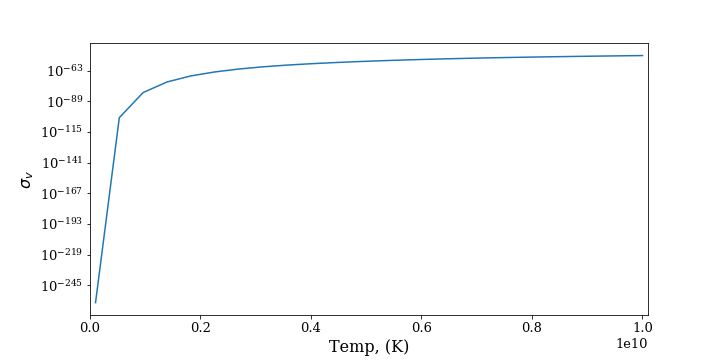
\includegraphics[width=0.8\linewidth]{xe130-cs130}}
	\caption{Сечение для СБР при столкновении $^{130}Xe$ с протоном}
	\label{ris:1}
\end{figure}

Важно отметить, что при вычислении СБР в начале искомого отрезка температуры ($\text{~}10^8\text{с}$), возникали ситуации деления на очень малый аргумент. Из-за этого на граничной слева температуре построенное сечение нельзя назвать точным из-за погрешностей округления, но поскольку, как мы знаем, SkyNet игнорирует реакции с небольшим сечением для даной температуры, данные погрешности не имеют смысла из-за пренебрежимо малого сечения ($\ll 10^{-100} \frac{\text{см}^2}{\text{с}}$).

\section{Анализ результатов}
В данной работе мы построили сечение СБР для столкновения всех элементов из таблицы (\ref{Tels}) с протоном (рис. \ref{ris:sigma-full}, \ref{ris:sigma-full-2}).

\begin{sidewaysfigure}
 	\center{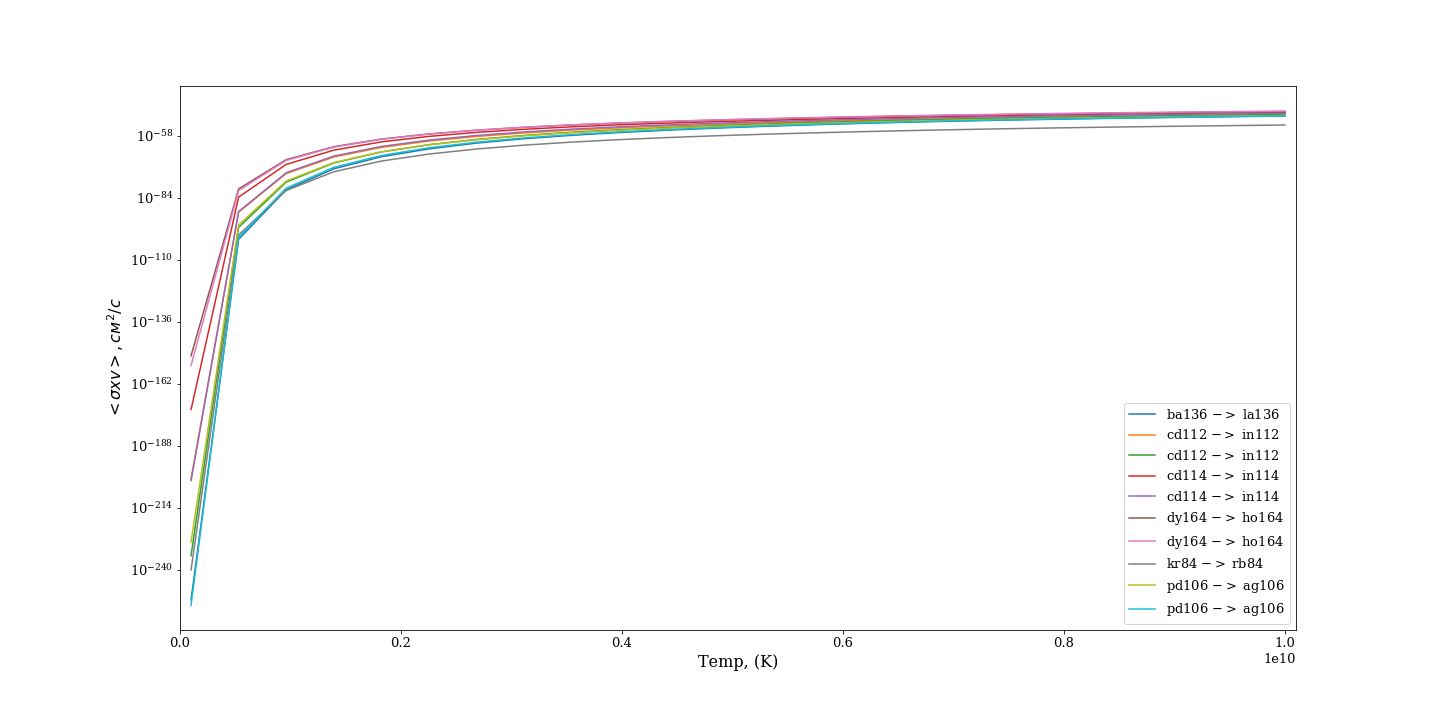
\includegraphics[width=1\linewidth]{sigma-full}}
 	\caption{Сечение для СБР при столкновении ядер ($^{136}Ba, ^{112}Cd, ^{114}Cd, ^{164}Dy, ^{84}Kr, ^{106}Pd$) с протоном}
 	\label{ris:sigma-full}
\end{sidewaysfigure}
\begin{sidewaysfigure}
	\center{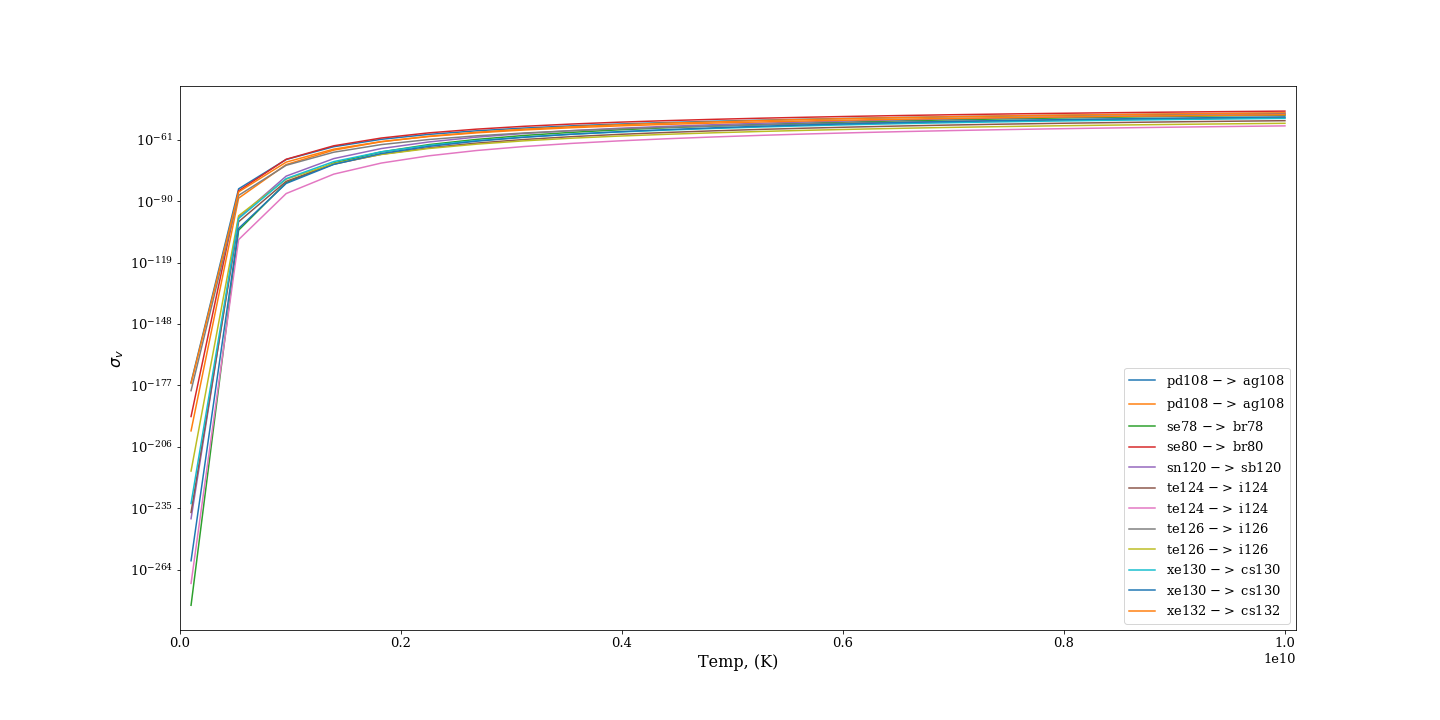
\includegraphics[width=1\linewidth]{sigma-full-2}}
	\caption{Сечение для СБР при столкновении ядер ($^{108}Pd, ^{78}Se, ^{80}Se, ^{120}Sn, ^{124}Te, ^{126}Te, ^{130}Xe, ^{132}Xe$) с протоном}
	\label{ris:sigma-full-2}
\end{sidewaysfigure}

Полученные 24 значения температур являются избыточными в нашем случае, так целью является параметризация данной зависимости через 7 параметров $a_0, ..., a_6$ (\ref{eq:system}). То есть мы имеет 17 лишних уравнений. Поэтому для решения переопределенной системы воспользуемся методом наименьших квадратов (\ref{ris:2}).

\begin{figure}[h]
	\center{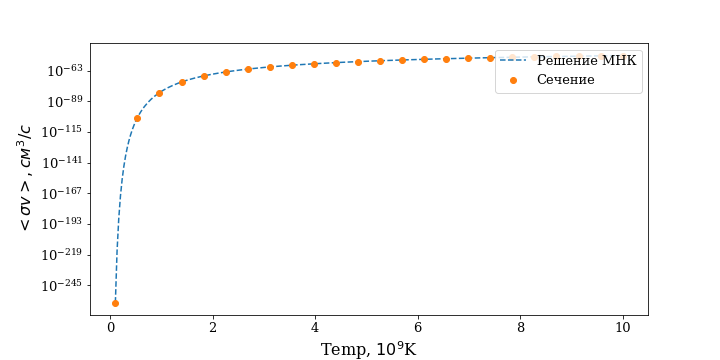
\includegraphics[width=0.8\linewidth]{compare-xe130-cs130}}
	\caption{Сравнение решения методов наименьших квадратов с полученным сечением}
	\label{ris:2}
\end{figure}

Далее, составим необходимый для REACLIB файл библиотеки реакций. Для перехода $^{130}Xe \to ^{130}Cs$ получаем строки вида: 

\begin{lstlisting}[label={lst:label}]
	5
	         pxe130cs130    p                  cleaw     0.00000e+00          
	 3.631089e+01-2.513083e+01-3.379005e+02 1.434772e+02                      
	-2.028014e+00-6.306473e-02-1.208779e+02                                   
	
\end{lstlisting}

В данном файле стоит отметить факт явного указания $p$ - протона в качестве участника реакции, так как сечение СБР зависит от концентрации протонов. 

Построим также графическое представление параметров $a$ для всех перечисленных в таблице (\ref{Tels}) реакций  (рис. \ref{ris:a-1} - \ref{ris:a-4}).

\begin{sidewaysfigure}
	\center{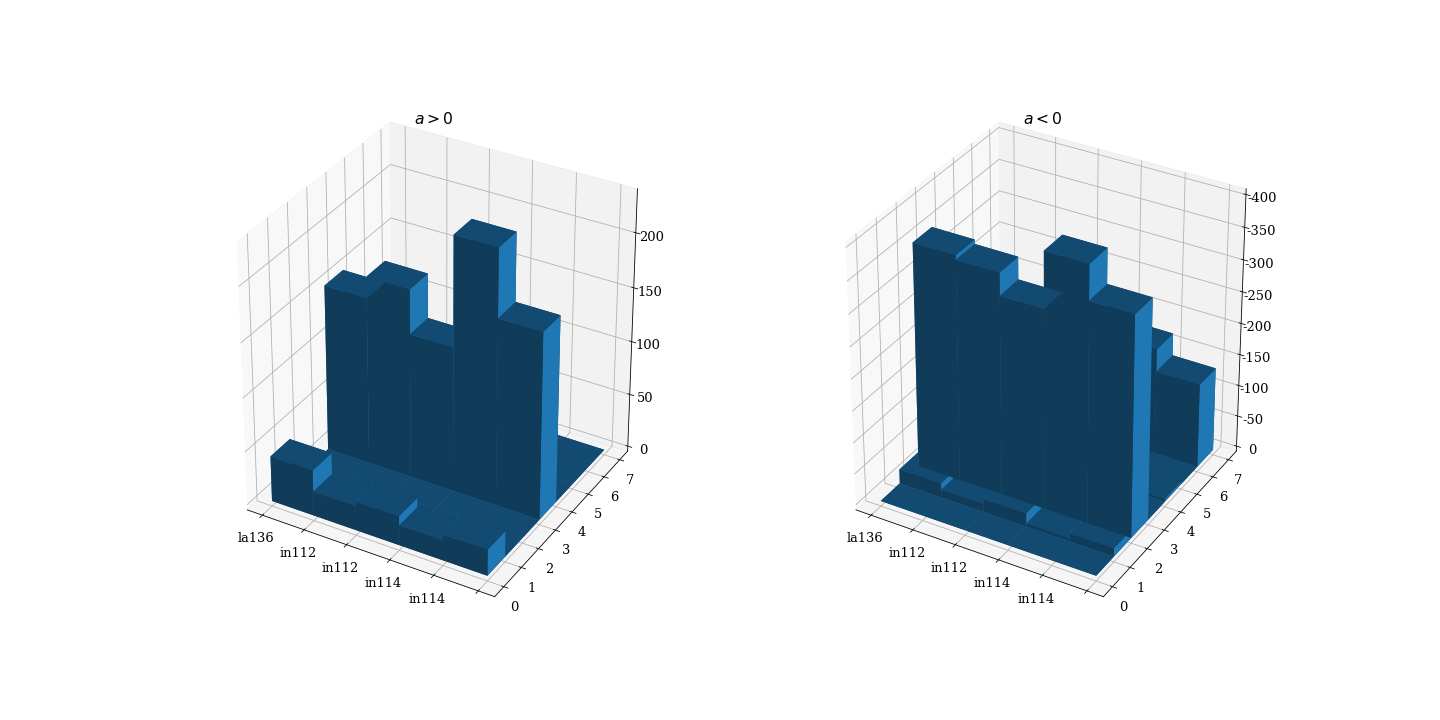
\includegraphics[width=1\linewidth]{a-1}}
	\caption{Значения параметров $a$ для столкновения протона с $^{136}Ba, ^{112}Cd, ^{114}Cd$}
	\label{ris:a-1}
\end{sidewaysfigure}
\begin{sidewaysfigure}
	\center{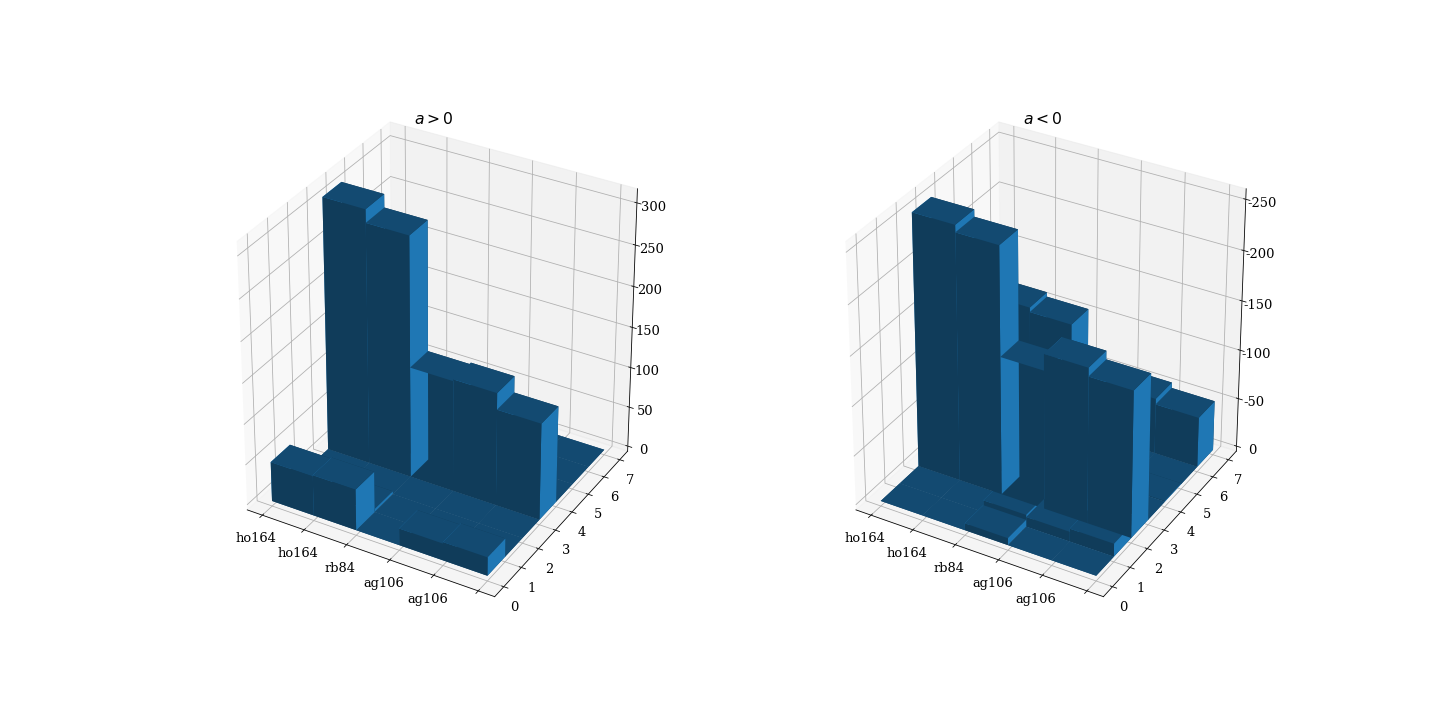
\includegraphics[width=1\linewidth]{a-2}}
	\caption{Значения параметров $a$ для столкновения протона с $^{164}Dy, ^{84}Kr, ^{106}Pd$}
	\label{ris:a-2}
\end{sidewaysfigure}
\begin{sidewaysfigure}
	\center{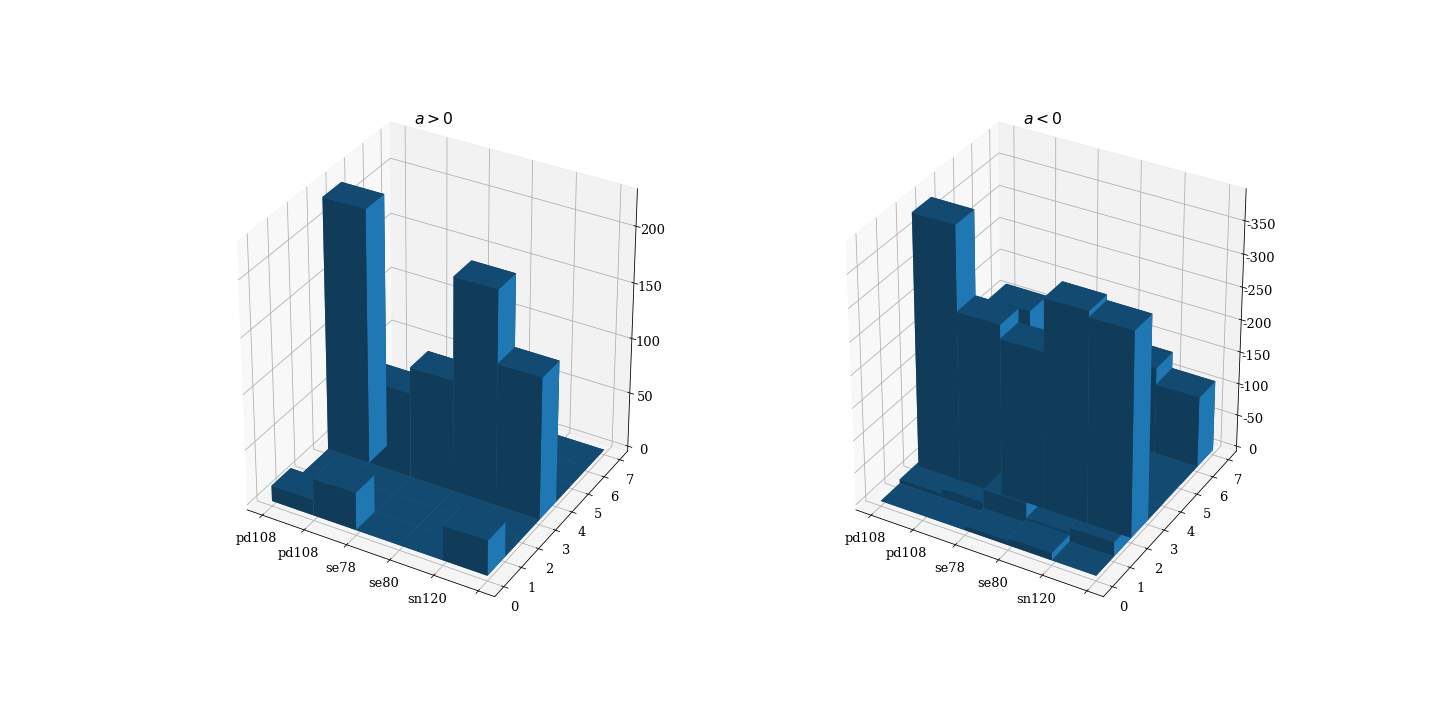
\includegraphics[width=1\linewidth]{a-3}}
	\caption{Значения параметров $a$ для столкновения протона с $^{108}Pd, ^{78}Se, ^{80}Se, ^{120}Sn$}
	\label{ris:a-3}
\end{sidewaysfigure}
\begin{sidewaysfigure}
	\center{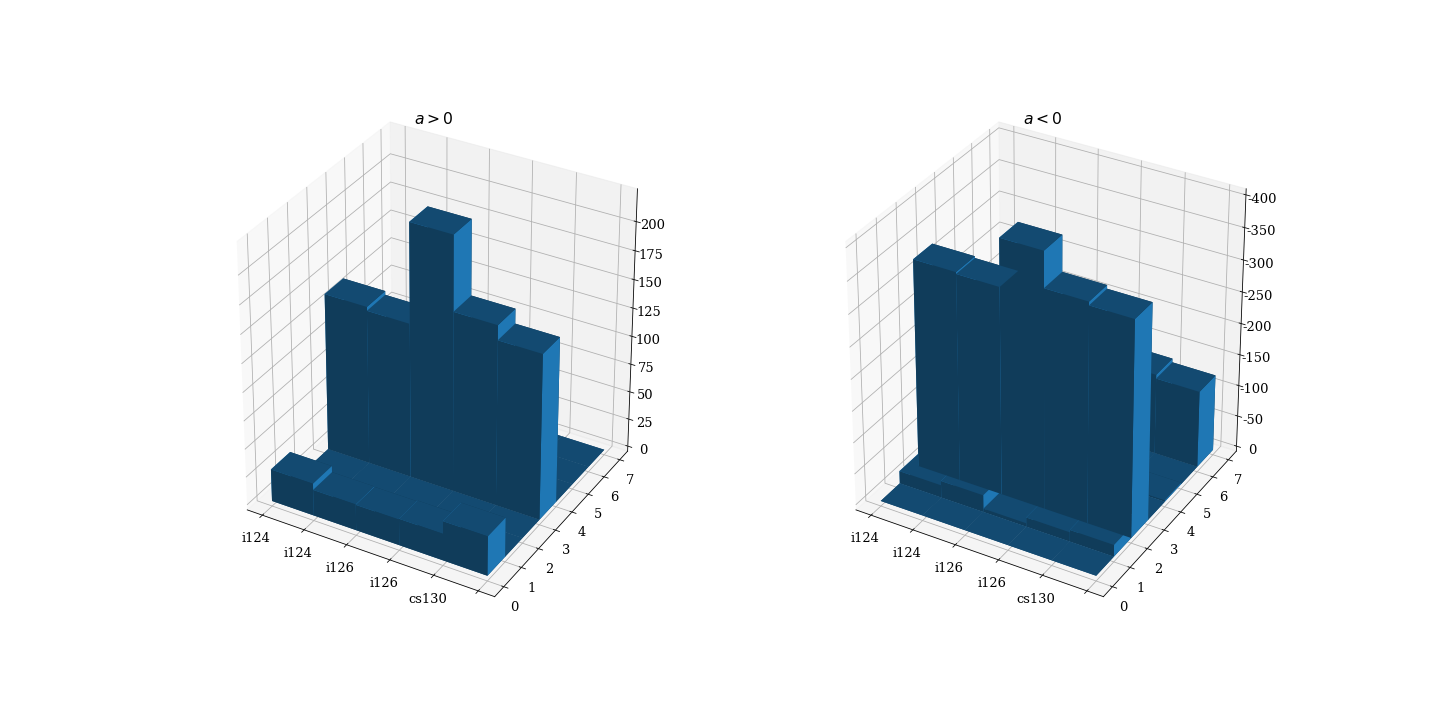
\includegraphics[width=1\linewidth]{a-4}}
	\caption{Значения параметров $a$ для столкновения протона с $^{124}Te, ^{126}Te, ^{130}Xe$}
	\label{ris:a-4}
\end{sidewaysfigure}

Для моделирования ядерных реакций воспользуемся включенной в SkyNet моделю r-process. Она содержит список из 7836 ядер, участвующих в реакциях, начальные распространенности этих ядер, а также зависимости плотности и температуры от времени. Эволюция протекает в промежутке времени от $1.21\times 10^{-3}c$ до $5\times 10^8c$. 

Изначально, если оставлять файл JINA REACLIB в таком виде, в котором он присутствует в библиотеке, влияние добавленных мною реакций отсутствовало. Это связано с тем, что в сети уже присутствовали реакции с этими элементами, но гораздо большим сечением, которое перекрывает наши реакции. Добится хоть какого-то влияния на небольших температурах невозможно, так как по характеру графика на рисунке (\ref{ris:1}) можно заметить его быстрое затухание при стремлении температуры справа к $10^8 K$, а именно при относительно низких ($10^9 K$) температурах протекает большая часть эволюции.

Для того, что проверить влияние, было решено учесть только те реакции, приводящие к образованию обойденных ядер, которые представляют из себя разрешенный $\beta$-распад. Для этого из библиотеки REACLIB были исключены реакции вида (\ref{eq:remove1}), то есть 168 реакций.

\begin{equation}
\label{eq:remove1}
	^{79}Br \to ^{78}Br + n
\end{equation}

Полученные данные представляют из себя иерархический формат данных h5. Извлекая конечные распространенности, видим результат для всех обойденных ядер (рис. \ref{ris:result}):

\begin{sidewaysfigure}[h]
	\center{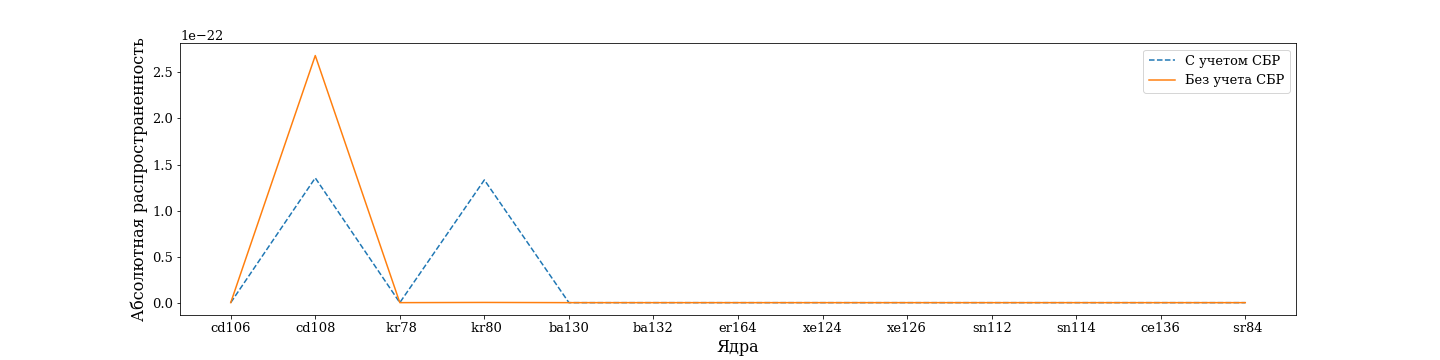
\includegraphics[width=1\linewidth]{result}}
	\caption{Конечные распространенности обойденных ядер}
	\label{ris:result}
\end{sidewaysfigure}

Построим график относительной ошибки между эволюцией элементов с нашей библиотекой реакций и тем, что присутствовало в изначальной версии REACLIB (рис. \ref{ris:result-err}):

\begin{sidewaysfigure}[h]
	\center{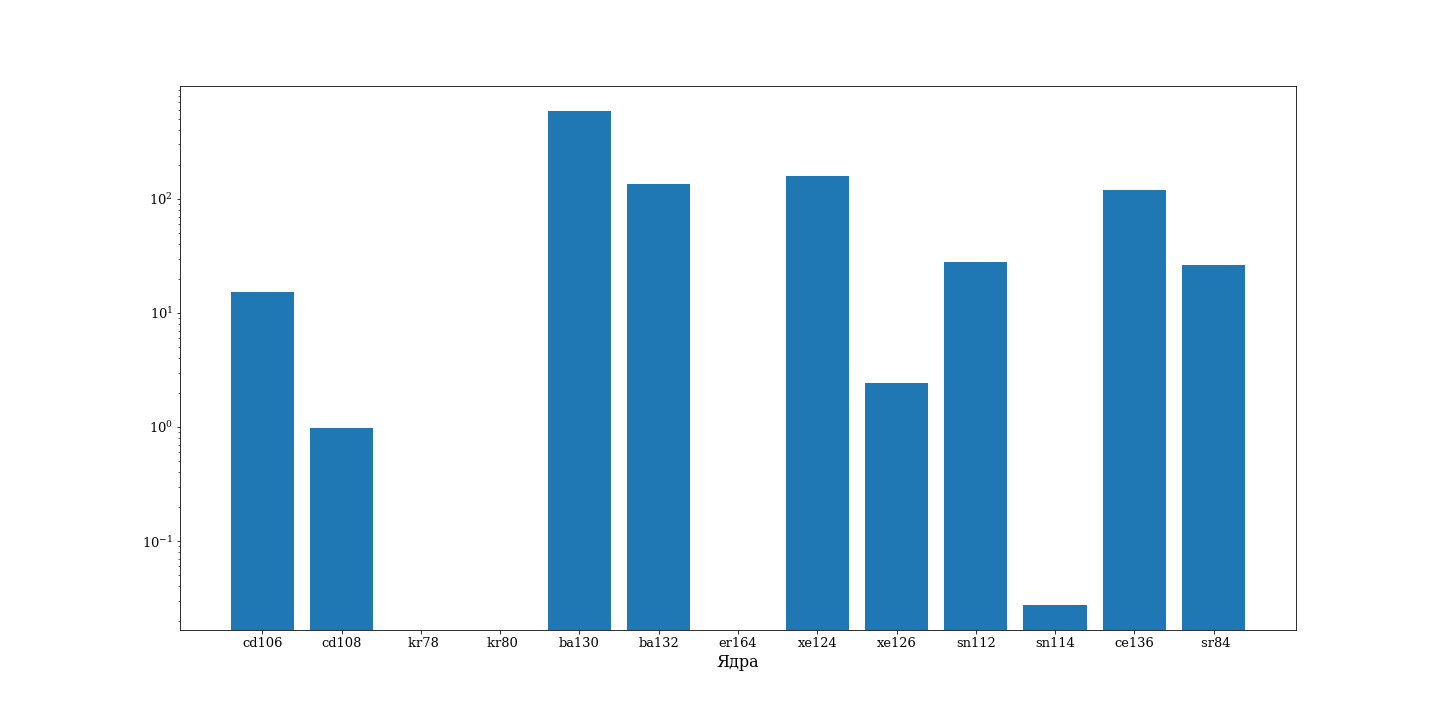
\includegraphics[width=1\linewidth]{result-err}}
	\caption{Относительная ошибка при сравнении стандартной библиотеки реакций SkyNet и библиотеки, учитывающей только СБР для образования обойденных изотопов}
	\label{ris:result-err}
\end{sidewaysfigure}

С учетом того, что мы полностью удалили все реакции, приводящие к возникновению обойденных $\beta$ ядер из сети реакций, полученная разница в их распространенностях оказалась не так велика, что говорит о том, что наши реакции действительно учитывались и смогли смоделировать возникновение некоторого количества обойденных ядер.

\section{Заключение}

В данной работе было рассмотрено влияние столкновительного бета распада на эволюцию звездных процессов. На языке Python был получено сечения для столкновительного процесса некоторых ядер с протоном. При помощи программного пакета SkyNet, а также дополнения библиотеки JINA REACLIB было подтверждено, что СБР может являться источником обойденных ядер и при больших значениях сечения это влияние существенно, но конкретно для ситуации столкновения с протоном, это влияние невелико даже для r-процесса. Чтобы увидеть эти изменения, пришлось учесть только реакции, приводящие к образованию обойденных ядер, которые представляют из себя разрешенный $\beta$-распад

Данная работа рассматривает только часть образований материнских ядер, причем при столкновении с протоном. Также, для расширения списка реакций необходимо добавить столкновительные реакции для других ядер, а также нейтронов, сечения для которых намного выше, ввиду отсутствия Кулоновского барьера.

\bibliographystyle{utf8gost705u}
\bibliography{sample}
\end{document} 